\documentclass[11pt,a4paper]{article}
\usepackage[margin=2cm]{geometry}
\usepackage{amsmath,amssymb}
\usepackage{tcolorbox}
\usepackage{booktabs}
\usepackage{enumitem}
\usepackage{hyperref}
\usepackage{xcolor}
\usepackage{fancyhdr}
\usepackage{tikz}
\usetikzlibrary{automata, positioning, arrows.meta}
\usepackage{listings}
\usepackage{adjustbox}

\tcbuselibrary{breakable,skins}

\newcommand{\fitmath}[1]{\begin{adjustbox}{max width=\linewidth}$\displaystyle #1$\end{adjustbox}}

\lstset{
  basicstyle=\ttfamily\small,
  breaklines=true,
  breakatwhitespace=false,
  breakautoindent=true,
  postbreak=\mbox{\textcolor{gray}{$\hookrightarrow$}\space},
  columns=fullflexible,
  keepspaces=true,
  xleftmargin=0pt,
  xrightmargin=0pt,
  aboveskip=4pt,
  belowskip=4pt,
  frame=none,
  commentstyle=\color{gray},
}

\newtcolorbox{definitionbox}[1]{colback=blue!5, colframe=blue!60!black,
  fonttitle=\bfseries, title=#1, breakable, enhanced jigsaw}

\newtcolorbox{conceptbox}[1]{colback=red!5, colframe=red!60!black,
  fonttitle=\bfseries, title=#1, breakable, enhanced jigsaw}

\newtcolorbox{examplebox}[1]{colback=green!5, colframe=green!50!black,
  fonttitle=\bfseries, title=#1, breakable, enhanced jigsaw}

\newtcolorbox{notebox}[1]{colback=orange!5, colframe=orange!60!black,
  fonttitle=\bfseries, title=#1, breakable, enhanced jigsaw}

\newcommand{\kemark}{\textcolor{red!70!black}{\textbf{[EXAM-RELEVANT]}}}
\newcommand{\kbg}{\textcolor{gray}{\textbf{[BACKGROUND]}}}
\newcommand{\kt}[1]{\par\vspace{0.3em}\colorbox{yellow!60}{\parbox{\dimexpr\linewidth-2\fboxsep}{#1}}\vspace{0.3em}}

\pagestyle{fancy}
\fancyhf{}
\lhead{AC Lecture 2 --- Cheatsheet}
\rhead{Jawad M.K. Qayyum}
\rfoot{\thepage}

\setlength{\parindent}{0pt}
\setlength{\parskip}{0.4em}

\begin{document}

\begin{center}
{\Huge\bfseries AC Lecture 2}\\[0.5em]
{\LARGE The Church-Turing Thesis}\\[0.3em]
{\large The Complete Guide to ``Why Turing Machines Are Enough''}\\[1em]
{\normalsize Algorithms and Computability --- Semester 6}\\
{\normalsize Cheatsheet for split-view study with slides}
\end{center}

\vspace{1em}
\tableofcontents
\newpage

%###############################################################################
%###############################################################################
\section{The Big Picture}
%###############################################################################
%###############################################################################

%-------------------------------------------------------------------------------
\subsection{Quick L1 Recap --- What We Already Know}

In Lecture 1 we established the foundations:

\begin{itemize}[nosep]
\item A \textbf{decision problem} is a language $L \subseteq \Sigma^*$ --- a set of strings we want to accept/reject.
\item A \textbf{Turing machine} (TM) is $M = (Q, \Sigma, \Gamma, \delta, s, t, r)$: a finite-state controller with an infinite tape and a read/write head.
\item A \textbf{configuration} $[q, \tau, \ell]$ is a complete snapshot: current state $q$, tape contents $\tau$, head position $\ell$.
\item A TM \textbf{decides} $L$ if it always halts, accepting exactly the strings in $L$.
\item A TM \textbf{recognises} $L$ if it accepts exactly $L$ (may loop on non-members).
\end{itemize}

The critical machinery we will reuse in every section of this lecture:
\begin{itemize}[nosep]
\item The transition function $\delta(q, a) = (q', b, d)$: ``In state $q$ reading symbol $a$, write $b$, move direction $d$, go to state $q'$.''
\item The step relation $\alpha \vdash \alpha'$: configuration $\alpha$ yields $\alpha'$ in one step.
\item The run $\alpha_0 \vdash \alpha_1 \vdash \alpha_2 \vdash \cdots$ on input $w$.
\end{itemize}

%-------------------------------------------------------------------------------
\subsection{The Problem: Why TMs Seem Too Weak}

\begin{conceptbox}{The Worry About Turing Machines}
After Lecture 1, you might think: ``A TM has one tape and one head. Real computers have RAM, multiple cores, internet access. Surely a TM can't do everything a real computer does?''

This is the central question of Lecture 2. Consider this concrete problem:

\textbf{The $w\#w$ problem:} Given a string like \texttt{011\#011}, accept it if the part before \texttt{\#} equals the part after \texttt{\#}. Reject otherwise.

With one tape, you would have to zig-zag back and forth across the \texttt{\#}, matching one symbol at a time, marking what you have seen. It is painful and slow.

With \textbf{two tapes}, you would simply copy the left part to tape 2, skip past \texttt{\#} on tape 1, and compare both tapes in parallel. Clean, fast, obvious.

So does adding more tapes make TMs \textit{strictly more powerful}? Can a 2-tape machine decide languages that a 1-tape machine \textit{cannot}?

\textbf{The answer is no.} And proving that is what this entire lecture is about.
\end{conceptbox}

%-------------------------------------------------------------------------------
\subsection{The Running Examples We Will Use}

Throughout this lecture, we thread two examples everywhere:

\begin{examplebox}{Running Example 1: The $w\#w$ Language}
\fitmath{L_{w\#w} = \{w\#w \mid w \in \{0,1\}^*\}}

Concrete test cases:
\begin{itemize}[nosep]
\item \texttt{011\#011} $\in L_{w\#w}$ (both sides match)
\item \texttt{01\#10} $\notin L_{w\#w}$ (both sides differ)
\item \texttt{0\#01} $\notin L_{w\#w}$ (different lengths)
\end{itemize}

We will build a 2-tape TM for this, then simulate it on a single tape.
\end{examplebox}

\begin{examplebox}{Running Example 2: The ``contains 110'' Language}
\fitmath{L_{110} = \{w \in \{0,1\}^* \mid w \text{ contains } 110 \text{ as a substring}\}}

Concrete test cases:
\begin{itemize}[nosep]
\item \texttt{0110} $\in L_{110}$ (contains 110 starting at position 2)
\item \texttt{1101} $\in L_{110}$ (contains 110 starting at position 1)
\item \texttt{0010} $\notin L_{110}$ (no 110 substring anywhere)
\end{itemize}

We will build a \textbf{nondeterministic} TM for this --- our first NTM.
\end{examplebox}

%-------------------------------------------------------------------------------
\subsection{This Lecture's Solution}

\begin{notebox}{The One-Line Summary}
\textbf{Lecture 2's answer:} Every ``reasonable'' extension of TMs (extra tapes, nondeterminism, stay-option, doubly-infinite tape) can be \textbf{simulated} by a standard 1-tape DTM. Therefore TMs are \textbf{robust}: they capture exactly the ``computable'' --- no more, no less. This claim is the \textbf{Church-Turing Thesis}.
\end{notebox}

\newpage

%###############################################################################
%###############################################################################
\section{The Church-Turing Thesis}
%###############################################################################
%###############################################################################

%-------------------------------------------------------------------------------
\subsection{What the Thesis Says}

\begin{notebox}{Analogy: The Universal Measuring Stick}
Imagine you are in ancient times and every village has its own unit of length --- one village uses ``arm lengths,'' another uses ``foot lengths,'' another uses ``horse strides.'' They are all different, but they all measure the same physical reality: actual distance.

Then someone proposes the \textbf{meter}. They claim: ``Everything that can be measured as a length can be expressed in meters. No matter what weird unit you invent, you can always convert it to meters.''

That is the Church-Turing Thesis for computation:
\begin{itemize}[nosep]
\item \textbf{Meters} = Turing machines.
\item \textbf{Arm lengths, foot lengths, horse strides} = Java, Python, multi-tape TMs, nondeterministic TMs, lambda calculus, \ldots
\item The claim: \textbf{every reasonable system of computation can compute exactly the same set of functions as a Turing machine.}
\end{itemize}

In our formal world: ``measuring distance'' = computing a function; ``meters'' = Turing machines; ``other units'' = other computational models.
\end{notebox}

\begin{conceptbox}{The Church-Turing Thesis \kbg}

\textbf{Plain English:}
Everything that can be computed (by any reasonable method whatsoever) can be computed by a Turing machine. There is no ``super computer'' that can solve problems TMs cannot.

\textbf{The Thesis (as stated in the course):}

\begin{quote}
\textit{Everything that is computable (in an intuitive sense) is computable by a Turing machine.}
\end{quote}

\textbf{Critical distinction --- thesis vs.\ theorem:}
\begin{itemize}[nosep]
\item A \textbf{theorem} is a statement that can be formally \textbf{proved}.
\item A \textbf{thesis} is a \textbf{claim} that cannot be proved --- because the term ``intuitively computable'' has no formal definition.
\item The Church-Turing Thesis is a thesis. It could theoretically be \textit{refuted} (by finding a reasonable model that computes something TMs cannot), but no one has done so in 90 years.
\end{itemize}

\kt{The Church-Turing Thesis is a claim, not a theorem. It says TMs capture ALL of computation. It cannot be proved, but it can (in principle) be refuted. No one has refuted it.}
\end{conceptbox}

\textbf{Historical note} \kbg: In the 1930s, Turing (Turing machines), Church (lambda calculus), and G\"odel (recursive functions) independently defined ``computable'' --- and all three definitions turned out to be equivalent. This convergence from three different directions is strong evidence for the thesis, but it is not a proof. The Entscheidungsproblem (Hilbert's ``decision problem'') asked whether there exists an algorithm that can decide the truth of any mathematical statement; Turing and Church independently showed the answer is \textbf{no}. That result required first defining what ``algorithm'' means --- which is what TMs are for.

%-------------------------------------------------------------------------------
\subsection{Turing-Completeness} \label{sec:turingcomplete}

\begin{notebox}{Analogy: Speaking Every Language}
Imagine a translator who can translate \textbf{from any language into English}. Whatever you say in French, Mandarin, Swahili --- they can express the same thing in English.

A \textbf{Turing-complete} system is the opposite direction: it is a system so powerful that \textbf{a Turing machine can be simulated inside it}. If you can build a TM inside your system, then your system can compute everything a TM can. Combined with the Church-Turing Thesis, that means your system can compute \textbf{everything that is computable}.

In our formal world: ``the translator'' = a simulation; ``English'' = Turing machines; ``your system being Turing-complete'' = your system can simulate every TM.
\end{notebox}

\begin{definitionbox}{Turing-Completeness \kbg}

\textbf{Plain English:}
A system is Turing-complete if it can simulate any Turing machine. That means it can compute anything a TM can compute.

\textbf{Formal:}
A computational system $S$ is \textbf{Turing-complete} if for every Turing machine $M$, there exists a program in $S$ that simulates $M$ (i.e., produces the same output on every input).

\textbf{Breaking Down the Notation:}
\begin{itemize}[nosep]
\item $S$ = any computational system (a programming language, a game, a spreadsheet, \ldots)
\item ``for every TM $M$'' = it is not enough to simulate one specific TM; you need to simulate \textbf{all} of them
\item ``simulates $M$'' = on every input $w$, if $M$ accepts/rejects/loops, the program in $S$ does the same
\end{itemize}

\textbf{Surprising examples of Turing-complete systems:}
\begin{itemize}[nosep]
\item Java, Python, C (obviously --- they are general-purpose languages)
\item \textbf{Microsoft Excel} (with enough formulas)
\item \textbf{Minecraft} (using redstone circuits)
\item \textbf{\LaTeX} (the typesetting system you are reading right now)
\item \textbf{Conway's Game of Life} (a simple 2D cellular automaton)
\item \textbf{Magic: The Gathering} (the card game)
\end{itemize}

\kt{Turing-completeness means a system can simulate any TM. Most programming languages (and some surprising non-programming systems) are Turing-complete.}
\end{definitionbox}

%-------------------------------------------------------------------------------
\subsection{Robustness of TMs} \label{sec:robustness}

\begin{notebox}{Analogy: The Indestructible Kitchen}
Imagine you have a basic kitchen: one stove, one knife, one pot. Someone says, ``Here, take a second stove, a blender, and a sous vide machine.'' You can now cook \textit{faster} and more \textit{conveniently} --- but can you cook \textit{new dishes} that were impossible before? No! With enough patience, you could make everything in the basic kitchen. The extra equipment makes you faster, not more capable.

In our formal world: ``basic kitchen'' = standard 1-tape TM; ``extra equipment'' = multi-tape, nondeterminism, stay-direction, doubly-infinite tape; ``new dishes'' = new decidable languages; ``faster cooking'' = fewer steps.
\end{notebox}

\begin{conceptbox}{Robustness of Turing Machines \kemark}

\textbf{Plain English:}
No matter how you ``upgrade'' a Turing machine --- give it extra tapes, let it stay put, let it guess nondeterministically, give it a tape that extends infinitely in both directions --- it can \textbf{never decide more languages} than a standard 1-tape deterministic TM. The extensions make TMs more convenient and sometimes faster, but never more powerful in terms of what they can compute.

\textbf{Why this matters:}
If we can show that every extension can be simulated by a standard TM, then the definition of ``computable'' does not depend on which variant of TM we use. This is the technical evidence for the Church-Turing Thesis.

\textbf{The four extensions we study in this lecture:}
\begin{enumerate}[nosep]
\item \textbf{Stay direction} ($d = 0$): head can stay in place (Section 3)
\item \textbf{Multi-tape}: $k$ tapes with $k$ independent heads (Section 4)
\item \textbf{Nondeterminism}: transition returns a \textit{set} of possible moves (Section 5)
\item \textbf{Doubly-infinite tape}: tape extends infinitely in both directions (Section 6)
\end{enumerate}

For each one, we prove: ``A standard 1-tape DTM can simulate this extension.''

\kt{Robustness = every reasonable extension of TMs can be simulated by a standard TM. The extensions add convenience, not power. This is the key evidence for the Church-Turing Thesis.}
\end{conceptbox}

%-------------------------------------------------------------------------------
\subsection{Outcome-Simulation} \label{sec:outcomesim}

\begin{notebox}{Analogy: Two Cooks Making the Same Dish}
Cook A uses a recipe with 10 steps. Cook B uses a different recipe with 47 steps. They use different ingredients and techniques. But if they start with the same raw food and always end up with the same final dish (or both fail to finish), we say Cook B \textbf{simulates} Cook A's outcome.

We do not care \textit{how} they cook --- only that the final result is the same: same dish produced, same failure mode.

In our formal world: ``Cook A'' = the fancy TM (multi-tape, NTM, \ldots); ``Cook B'' = the standard 1-tape DTM; ``same dish'' = same accept/reject outcome; ``both fail to finish'' = both loop.
\end{notebox}

\begin{definitionbox}{Outcome-Simulation \kemark}

\textbf{Plain English:}
Machine $M'$ outcome-simulates machine $M$ if they always give the same answer. If $M$ accepts, $M'$ accepts. If $M$ rejects, $M'$ rejects. If $M$ loops forever, $M'$ may also loop (but it must not suddenly accept or reject).

\textbf{Formal Definition:}
$M'$ \textbf{outcome-simulates} $M$ if for every input $w \in \Sigma^*$:
\begin{enumerate}[nosep]
\item If $M$ halts on $w$, then $M'$ halts on $w$.
\item $M$ accepts $w$ if and only if $M'$ accepts $w$.
\end{enumerate}

\textbf{Breaking Down the Notation:}
\begin{itemize}[nosep]
\item $M$ = the machine being simulated (the ``fancy'' one)
\item $M'$ = the simulator (the ``standard'' one)
\item ``halts'' = reaches $t$ (accept) or $r$ (reject), does not loop forever
\item Condition 1 says: $M$ halting $\Rightarrow$ $M'$ halting (if $M$ finishes, $M'$ must finish too)
\item Condition 2 says: they agree on accept/reject (same final answer)
\item Together: if $M$ accepts, $M'$ accepts. If $M$ rejects, $M'$ rejects. If $M$ loops, $M'$ may loop.
\end{itemize}

\textbf{What about the case where $M$ loops?}
The definition is deliberately silent. If $M$ loops on input $w$, $M'$ is allowed to do anything --- loop, halt, whatever. The only guarantee is in the direction where $M$ halts.

\textbf{Why ``outcome'' simulation?} Because we only care about the \textit{outcome} (accept/reject/loop), not the intermediate configurations. $M'$ can use a completely different tape contents, different states, take a different number of steps --- as long as the final answer matches.

\kt{Outcome-simulation: $M'$ simulates $M$ if whenever $M$ halts, $M'$ halts too, and they always agree on accept vs.\ reject. The intermediate computation can be completely different.}
\end{definitionbox}

\begin{examplebox}{Concrete Example of Outcome-Simulation}
Suppose $M$ is a 2-tape TM that decides $L_{w\#w}$ (our running example). We want to build $M'$, a standard 1-tape DTM, that outcome-simulates $M$.

We need:
\begin{itemize}[nosep]
\item On input \texttt{011\#011}: $M$ accepts (both sides match), so $M'$ must also accept.
\item On input \texttt{01\#10}: $M$ rejects (sides differ), so $M'$ must also reject.
\item On input \texttt{0\#01}: $M$ rejects (different lengths), so $M'$ must also reject.
\end{itemize}

$M'$ does not need to use the same algorithm. It does not need to have two tapes. It just needs to give the same yes/no answer on every input. In Section 4, we will build exactly this $M'$.
\end{examplebox}

\newpage

%###############################################################################
%###############################################################################
\section{Robustness in Action: The Stay Direction}
%###############################################################################
%###############################################################################

%-------------------------------------------------------------------------------
\subsection{The Extension: What ``Stay'' Means}

\begin{notebox}{Analogy: The Third Gear Option}
Imagine you are driving a car that can only go forward or reverse. Now someone adds a ``park'' gear --- you can stay in place. Does this let you reach new destinations? No! Anywhere you could reach by driving forward and reverse, you can still reach. The park gear just means you do not have to jiggle forward-then-backward when you want to stay put.

In our formal world: ``forward'' = move right ($+1$); ``reverse'' = move left ($-1$); ``park gear'' = stay ($0$); ``destinations'' = decidable languages.
\end{notebox}

\begin{definitionbox}{TM with Stay Direction \kemark}

\textbf{Plain English:}
A standard TM's transition function outputs a direction $d \in \{-1, +1\}$: move left or move right. A TM with the ``stay'' extension also allows $d = 0$: the head stays in place. Everything else is identical.

\textbf{Formal:}

Standard TM: $\delta: (Q \setminus \{t,r\}) \times \Gamma \to Q \times \Gamma \times \{-1, +1\}$

Stay-TM: $\delta: (Q \setminus \{t,r\}) \times \Gamma \to Q \times \Gamma \times \{-1, 0, +1\}$

\textbf{Breaking Down the Notation:}
\begin{itemize}[nosep]
\item $\{-1, 0, +1\}$ = the set of directions: left, \textbf{stay}, right
\item $d = 0$ means ``after writing, do not move the head at all''
\item Everything else (states, tape alphabet, accept/reject states) is unchanged
\end{itemize}

\kt{A Stay-TM is identical to a standard TM except the head can also stay in place ($d = 0$) instead of moving left or right.}
\end{definitionbox}

%-------------------------------------------------------------------------------
\subsection{The Simulation Construction}

\begin{conceptbox}{The Key Idea: Replace ``Stay'' with ``Right Then Left'' \kemark}

\textbf{The insight:} If the head needs to stay at position $\ell$, we can instead:
\begin{enumerate}[nosep]
\item Move right to position $\ell + 1$ (entering a temporary auxiliary state).
\item Immediately move left back to position $\ell$ (without changing the tape at position $\ell + 1$).
\end{enumerate}

After these two moves, the head is back at position $\ell$, the tape is unchanged at position $\ell + 1$ (we read whatever was there and write it back), and we are in the correct target state. Net effect: identical to staying.

\textbf{The problem:} We need an extra state for the ``in between'' moment (at position $\ell+1$, about to move back). This auxiliary state must be unique per target state to avoid conflicts.
\end{conceptbox}

\begin{definitionbox}{Formal Construction: Simulating Stay \kemark}

\textbf{Given:} A Stay-TM $M = (Q, \Sigma, \Gamma, \delta, s, t, r)$ where $\delta$ can output $d = 0$.

\textbf{Construct:} A standard TM $M' = (Q', \Sigma, \Gamma, \delta', s, t, r)$ where $\delta'$ only outputs $d \in \{-1, +1\}$.

\textbf{Step 1: Expand the state set.}
For every state $q \in Q$, create an auxiliary state $q_L$ (think: ``$q$, but I need to move Left to finish the stay-simulation'').
\fitmath{Q' = Q \cup \{q_L \mid q \in Q\}}

\textbf{Step 2: Define the new transition function $\delta'$.}

\textbf{Case 1:} If the original transition does NOT stay ($d \neq 0$):
\fitmath{\text{If } \delta(q, a) = (q', b, d) \text{ with } d \in \{-1, +1\}, \text{ then } \delta'(q, a) = (q', b, d)}
(Copy it unchanged.)

\textbf{Case 2:} If the original transition stays ($d = 0$):
\fitmath{\text{If } \delta(q, a) = (q', b, 0), \text{ then:}}
\begin{enumerate}[nosep]
\item $\delta'(q, a) = (q'_L, b, +1)$ \quad (Write $b$, move right, enter auxiliary state)
\item $\delta'(q'_L, c) = (q', c, -1)$ for every $c \in \Gamma$ \quad (Read whatever is there, write it back unchanged, move left, enter the real target state)
\end{enumerate}

\textbf{Breaking Down the Notation:}
\begin{itemize}[nosep]
\item $q_L$ = auxiliary ``bounce-back'' state for state $q$. The subscript $L$ reminds us: ``I still need to move Left.''
\item In step (1), we do the write ($b$) and move right instead of staying.
\item In step (2), $c$ is whatever symbol happens to be at position $\ell+1$. We do not know what $c$ is, so we define $\delta'(q'_L, c)$ for \textit{every} possible $c \in \Gamma$. We write $c$ back (no change) and move left.
\item After both steps, the head is back at position $\ell$, the tape is correct, and we are in state $q'$. Identical outcome to staying.
\end{itemize}

\kt{Simulate ``stay'' by: (1) write the new symbol, move right to auxiliary state $q'_L$; (2) read the neighbor, write it back unchanged, move left to real target state $q'$. The head returns to its original position.}
\end{definitionbox}

%-------------------------------------------------------------------------------
\subsection{Full Worked Trace: Simulating a Stay Transition}

Let us build a tiny Stay-TM and trace the simulation step by step.

\begin{examplebox}{Setup: A Tiny Stay-TM}

\textbf{The machine $M$:} On input over $\{0, 1\}$, it reads the first symbol. If it is a $0$, it writes $X$ and \textbf{stays} (to re-read the same position), then accepts when it reads the $X$.

Formally:
\begin{itemize}[nosep]
\item $Q = \{s, q_1, t, r\}$, $\Sigma = \{0, 1\}$, $\Gamma = \{0, 1, X, \sqcup\}$
\item $\delta(s, 0) = (q_1, X, 0)$ \quad --- the \textbf{stay} transition
\item $\delta(q_1, X) = (t, X, +1)$ \quad --- accept
\end{itemize}

\textbf{Run on input \texttt{0}:}

\medskip
\begin{tabular}{ccl}
\toprule
Step & Config & Action \\
\midrule
0 & $[s,\ \underline{0}\sqcup, \ 0]$ & Read $0$ in state $s$. Apply $\delta(s,0) = (q_1, X, 0)$. \\
1 & $[q_1,\ \underline{X}\sqcup,\ 0]$ & Write $X$, \textbf{stay} at position 0, go to $q_1$. \\
  &                                     & Read $X$ in state $q_1$. Apply $\delta(q_1, X) = (t, X, +1)$. \\
2 & $[t,\ X\underline{\sqcup},\ 1]$ & Write $X$, move right, go to $t$. \textbf{Accept!} \\
\bottomrule
\end{tabular}

\medskip
(Here $\underline{a}$ marks the head position.)
\end{examplebox}

Now let us trace the \textbf{simulator} $M'$ (standard TM, no stay) on the same input.

\begin{examplebox}{Trace: The Simulator $M'$ on Input \texttt{0}}

\textbf{Construction applied:}
\begin{itemize}[nosep]
\item $Q' = \{s, q_1, t, r\} \cup \{s_L, (q_1)_L, t_L, r_L\}$ \quad (we add $q_L$ for every $q$, though only $(q_1)_L$ will actually be used)
\item The stay transition $\delta(s, 0) = (q_1, X, 0)$ becomes:
  \begin{enumerate}[nosep]
  \item $\delta'(s, 0) = ((q_1)_L, X, +1)$ \quad --- write $X$, move right, enter auxiliary state
  \item $\delta'((q_1)_L, c) = (q_1, c, -1)$ for every $c \in \Gamma$ \quad --- write back $c$, move left
  \end{enumerate}
\item The non-stay transition $\delta(q_1, X) = (t, X, +1)$ copies unchanged:
  \begin{itemize}[nosep]
  \item $\delta'(q_1, X) = (t, X, +1)$
  \end{itemize}
\end{itemize}

\textbf{Step-by-step trace on input \texttt{0}:}

\medskip
\begin{tabular}{cccl}
\toprule
Step & State & Tape (head underlined) & Action \\
\midrule
0 & $s$ & $\underline{0}\;\sqcup$ & Read $0$. Apply $\delta'(s, 0) = ((q_1)_L, X, +1)$. \\
1 & $(q_1)_L$ & $X\;\underline{\sqcup}$ & Wrote $X$ at pos 0, moved right to pos 1. \\
  &           &                         & Read $\sqcup$. Apply $\delta'((q_1)_L, \sqcup) = (q_1, \sqcup, -1)$. \\
2 & $q_1$ & $\underline{X}\;\sqcup$ & Wrote $\sqcup$ back at pos 1 (unchanged), moved left to pos 0. \\
  &       &                          & Read $X$. Apply $\delta'(q_1, X) = (t, X, +1)$. \\
3 & $t$ & $X\;\underline{\sqcup}$ & Wrote $X$ at pos 0 (unchanged), moved right. \textbf{Accept!} \\
\bottomrule
\end{tabular}

\medskip
\textbf{Comparison:}
\begin{itemize}[nosep]
\item Original $M$: 2 steps (step 0$\to$1 is the stay, step 1$\to$2 accepts).
\item Simulator $M'$: 3 steps (step 0$\to$1 moves right, step 1$\to$2 bounces back left, step 2$\to$3 accepts).
\item Same final answer (accept), same tape contents at the end. $M'$ just took one extra step to simulate the stay.
\end{itemize}
\end{examplebox}

%-------------------------------------------------------------------------------
\subsection{Why the Simulation Preserves Correctness}

\begin{conceptbox}{Correctness of the Stay Simulation \kemark}

We need to verify that $M'$ outcome-simulates $M$:

\textbf{1. Every non-stay transition is copied verbatim.} So those steps produce identical configurations.

\textbf{2. Every stay transition $\delta(q,a) = (q', b, 0)$ is replaced by two steps:}
\begin{itemize}[nosep]
\item After step 1: head is one position right, in auxiliary state $q'_L$, tape has $b$ at the original position.
\item After step 2: head is back at the original position, in state $q'$, tape has $b$ at the original position and the cell to the right is unchanged.
\end{itemize}
Net effect: same as staying. The configuration after the two-step simulation matches the configuration after the original stay --- same state ($q'$), same head position, same tape contents.

\textbf{3. No conflicts.} The auxiliary states $q_L$ are fresh --- they are not in the original $Q$. And in an auxiliary state, we immediately bounce back; we never ``linger'' in auxiliary states or chain them.

\textbf{4. Halting is preserved.} If $M$ reaches $t$ or $r$, then $M'$ also reaches $t$ or $r$ (just possibly after one extra step if the last transition was a stay). If $M$ loops, $M'$ loops too (each loop iteration in $M$ corresponds to at most 2 steps in $M'$).

\kt{The stay simulation is correct because each stay is replaced by exactly two moves (right then left) that restore the original head position and tape contents. The extra auxiliary states do not interfere with the original computation.}
\end{conceptbox}

\newpage

%###############################################################################
%###############################################################################
\section{Multi-Tape Turing Machines}
%###############################################################################
%###############################################################################

This is the biggest and most important section of the lecture. We spend a lot of time here because multi-tape TMs are both practically useful and the simulation technique is a key exam topic.

%-------------------------------------------------------------------------------
\subsection{Why We Want Multiple Tapes: The $w\#w$ Pain Point}

\begin{notebox}{Analogy: Comparing Two Documents}
Imagine you have two printed documents and you need to check if they are identical. With \textbf{one finger}, you would have to: read a word from document 1, memorize it, move your finger to document 2, find the corresponding word, compare, move back. Slow and error-prone.

With \textbf{two fingers} (one on each document), you just advance both fingers in sync, comparing word by word. Same task, massively simpler.

In our formal world: ``documents'' = parts of the input tape; ``fingers'' = tape heads; ``one finger'' = 1-tape TM; ``two fingers'' = 2-tape TM.
\end{notebox}

\begin{conceptbox}{The Problem with 1-Tape for $w\#w$ \kemark}

Consider the language $L_{w\#w} = \{w\#w \mid w \in \{0,1\}^*\}$ on a single-tape TM.

To check if \texttt{011\#011} is in $L_{w\#w}$ with one tape, you would need to:
\begin{enumerate}[nosep]
\item Read the first symbol of the left part (0). Mark it (e.g., overwrite with $X$).
\item Scan right past \# to find the first unmarked symbol of the right part.
\item Compare. If they match, mark the right symbol.
\item Scan left past \# to find the next unmarked symbol on the left.
\item Repeat for every symbol.
\item Finally check that both sides are fully marked (same length).
\end{enumerate}

For an input of length $n$, you cross the \# separator $O(n)$ times, each crossing takes $O(n)$ steps. Total: $O(n^2)$ steps. And the machine is complicated --- many states just for bookkeeping.

\textbf{With two tapes, it is trivial:}
\begin{enumerate}[nosep]
\item Copy the left part to tape 2. (One pass.)
\item Skip past \# on tape 1. Rewind tape 2.
\item Compare tape 1 and tape 2 symbol by symbol. (One pass.)
\end{enumerate}

Total: $O(n)$ steps. Clean, simple, obvious.

\kt{Multiple tapes make some algorithms dramatically simpler and faster. The $w\#w$ language goes from $O(n^2)$ zig-zagging to $O(n)$ clean comparison.}
\end{conceptbox}

%-------------------------------------------------------------------------------
\subsection{The 2-Tape TM for $w\#w$: Conceptual View}

Let us design a 2-tape TM for $L_{w\#w}$ step by step.

\begin{examplebox}{Design: 2-Tape TM for $w\#w$}

\textbf{Setup:}
\begin{itemize}[nosep]
\item Tape 1: contains the input (e.g., \texttt{011\#011})
\item Tape 2: initially blank (all $\sqcup$)
\item Both heads start at position 0
\end{itemize}

\textbf{Phase 1: Copy $w$ to tape 2 (until we see \#)}
\begin{itemize}[nosep]
\item Read from tape 1. If the symbol is not \#, write it to tape 2. Advance both heads right.
\item When tape 1 reads \#, stop copying. Tape 2 now contains a copy of $w$.
\end{itemize}

\textbf{Phase 2: Rewind tape 2, advance tape 1 past \#}
\begin{itemize}[nosep]
\item Move tape 2's head all the way back to position 0 (rewind).
\item Move tape 1's head one step right (past the \#).
\item Now tape 1's head is at the first symbol of the right $w$, and tape 2's head is at the first symbol of the copied $w$.
\end{itemize}

\textbf{Phase 3: Compare symbol by symbol}
\begin{itemize}[nosep]
\item Read both tapes simultaneously.
\item If the symbols match, advance both heads right.
\item If they differ, \textbf{reject}.
\item If both reach blank ($\sqcup$) simultaneously, \textbf{accept} (same length, all symbols matched).
\item If one reaches blank before the other, \textbf{reject} (different lengths).
\end{itemize}
\end{examplebox}

\begin{center}
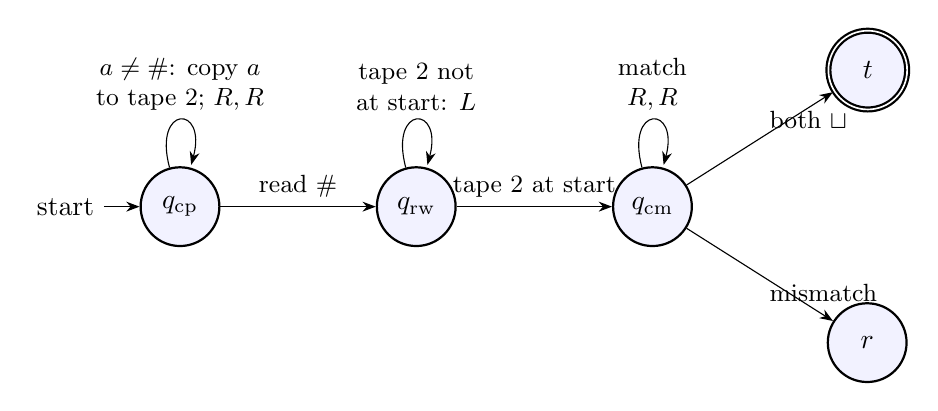
\begin{tikzpicture}[->, >=Stealth, node distance=3cm, every state/.style={thick, fill=blue!5, minimum size=1cm}]
    \node[state, initial] (copy) {$q_{\text{cp}}$};
    \node[state] (rew) [right of=copy] {$q_{\text{rw}}$};
    \node[state] (cmp) [right of=rew] {$q_{\text{cm}}$};
    \node[state, accepting] (acc) [above right=1cm and 2cm of cmp] {$t$};
    \node[state] (rej) [below right=1cm and 2cm of cmp] {$r$};

    \path (copy) edge [loop above] node[align=center, font=\small] {$a \neq \#$: copy $a$\\to tape 2; $R,R$} (copy)
          (copy) edge node[above, font=\small] {read $\#$} (rew)
          (rew) edge [loop above] node[align=center, font=\small] {tape 2 not\\at start: $L$} (rew)
          (rew) edge node[above, font=\small] {tape 2 at start} (cmp)
          (cmp) edge [loop above] node[align=center, font=\small] {match\\$R, R$} (cmp)
          (cmp) edge node[above right, font=\small] {both $\sqcup$} (acc)
          (cmp) edge node[below right, font=\small] {mismatch} (rej);
\end{tikzpicture}
\end{center}

%-------------------------------------------------------------------------------
\subsection{Full Trace of the 2-Tape Machine on \texttt{011\#011}}

\begin{examplebox}{{Complete Trace: 2-Tape TM on Input 011\#011}}

We show the state of \textbf{both tapes} at every step. The caret \texttt{\^{}} marks the head position on each tape.

\textbf{Initial configuration:}
\begin{lstlisting}
Tape 1: [0] [1] [1] [#] [0] [1] [1] [_]
          ^
Tape 2: [_] [_] [_] [_] [_] [_] [_] [_]
          ^
State: q_cp
\end{lstlisting}

\textbf{--- Phase 1: Copy $w$ to tape 2 ---}

\textbf{Step 1:} Read tape 1 = \texttt{0}, tape 2 = $\sqcup$. Since \texttt{0} $\neq$ \texttt{\#}: write \texttt{0} to tape 2, move both heads right.
\begin{lstlisting}
Tape 1: [0] [1] [1] [#] [0] [1] [1] [_]
              ^
Tape 2: [0] [_] [_] [_] [_] [_] [_] [_]
              ^
State: q_cp
\end{lstlisting}

\textbf{Step 2:} Read tape 1 = \texttt{1}. Since \texttt{1} $\neq$ \texttt{\#}: write \texttt{1} to tape 2, move both right.
\begin{lstlisting}
Tape 1: [0] [1] [1] [#] [0] [1] [1] [_]
                  ^
Tape 2: [0] [1] [_] [_] [_] [_] [_] [_]
                  ^
State: q_cp
\end{lstlisting}

\textbf{Step 3:} Read tape 1 = \texttt{1}. Since \texttt{1} $\neq$ \texttt{\#}: write \texttt{1} to tape 2, move both right.
\begin{lstlisting}
Tape 1: [0] [1] [1] [#] [0] [1] [1] [_]
                      ^
Tape 2: [0] [1] [1] [_] [_] [_] [_] [_]
                      ^
State: q_cp
\end{lstlisting}

\textbf{Step 4:} Read tape 1 = \texttt{\#}. This signals end of $w$. Move tape 1 right (past \#). Enter $q_{\text{rw}}$.
\begin{lstlisting}
Tape 1: [0] [1] [1] [#] [0] [1] [1] [_]
                          ^
Tape 2: [0] [1] [1] [_] [_] [_] [_] [_]
                      ^
State: q_rw
\end{lstlisting}

\textbf{--- Phase 2: Rewind tape 2 ---}

\textbf{Step 5:} Tape 2 head at position 3, reads $\sqcup$. Move tape 2 head left. (Tape 1 head stays.)
\begin{lstlisting}
Tape 1: [0] [1] [1] [#] [0] [1] [1] [_]
                          ^
Tape 2: [0] [1] [1] [_] [_] [_] [_] [_]
                  ^
State: q_rw
\end{lstlisting}

\textbf{Step 6:} Tape 2 at position 2, reads \texttt{1}. Not at start yet. Move left.
\begin{lstlisting}
Tape 1: ... same ...      ^  (pos 4)
Tape 2: [0] [1] [1] ...
              ^               (pos 1)
State: q_rw
\end{lstlisting}

\textbf{Step 7:} Tape 2 at position 1, reads \texttt{1}. Move left.
\begin{lstlisting}
Tape 1: ... same ...      ^  (pos 4)
Tape 2: [0] [1] [1] ...
          ^                   (pos 0)
State: q_rw
\end{lstlisting}

\textbf{Step 8:} Tape 2 at position 0 --- this is the start. Transition to $q_{\text{cm}}$.
\begin{lstlisting}
Tape 1: [0] [1] [1] [#] [0] [1] [1] [_]
                          ^               (pos 4)
Tape 2: [0] [1] [1] [_] [_] [_] [_] [_]
          ^                               (pos 0)
State: q_cm
\end{lstlisting}

\textbf{--- Phase 3: Compare ---}

\textbf{Step 9:} Tape 1 reads \texttt{0} (pos 4), tape 2 reads \texttt{0} (pos 0). Match! Both right.
\begin{lstlisting}
Tape 1: ... [#] [0] [1] [1] [_]
                      ^               (pos 5)
Tape 2: [0] [1] [1] [_] ...
              ^                       (pos 1)
State: q_cm
\end{lstlisting}

\textbf{Step 10:} Tape 1 reads \texttt{1} (pos 5), tape 2 reads \texttt{1} (pos 1). Match! Both right.
\begin{lstlisting}
Tape 1: ... [0] [1] [1] [_]
                      ^           (pos 6)
Tape 2: [0] [1] [1] [_] ...
                  ^               (pos 2)
State: q_cm
\end{lstlisting}

\textbf{Step 11:} Tape 1 reads \texttt{1} (pos 6), tape 2 reads \texttt{1} (pos 2). Match! Both right.
\begin{lstlisting}
Tape 1: ... [1] [1] [_]
                      ^       (pos 7)
Tape 2: [0] [1] [1] [_] ...
                      ^       (pos 3)
State: q_cm
\end{lstlisting}

\textbf{Step 12:} Tape 1 reads $\sqcup$ (pos 7), tape 2 reads $\sqcup$ (pos 3). \textbf{Both blank simultaneously!}

Transition to $t$. \textbf{ACCEPT!}

\medskip
\textbf{Result:} Input \texttt{011\#011} is \textbf{accepted} in 12 steps.
\end{examplebox}

\begin{examplebox}{Quick Trace: 2-Tape TM on Rejecting Input \texttt{01\#10}}

Following the same phases:

\textbf{Phase 1 (Copy):} Copy \texttt{01} to tape 2 (2 copy steps). See \#, advance tape 1.

After rewind, we are ready to compare:
\begin{lstlisting}
Tape 1: [0] [1] [#] [1] [0] [_]
                      ^               (pos 3)
Tape 2: [0] [1] [_] [_] ...
          ^                           (pos 0)
State: q_cm
\end{lstlisting}

\textbf{Phase 3 (Compare):}
\begin{itemize}[nosep]
\item Step: tape 1 reads \texttt{1} (pos 3), tape 2 reads \texttt{0} (pos 0). \textbf{Mismatch! REJECT.}
\end{itemize}

The machine rejects immediately at the first comparison. It does not need to check the whole string.
\end{examplebox}

%-------------------------------------------------------------------------------
\subsection{Formal Definition of $k$-Tape DTM}

\begin{notebox}{Analogy: A Chef with $k$ Cutting Boards}
A chef has $k$ cutting boards (tapes) and one hand on each board (heads). In each step, the chef looks at what is under each hand, then simultaneously: chops something on each board (writes) and moves each hand independently (left, stay, or right). Each board is independent, but the chef's brain (state) is shared across all boards.

In our formal world: ``cutting boards'' = tapes; ``hands'' = heads; ``chef's brain'' = state; ``chopping'' = writing; ``moving hands'' = moving heads.
\end{notebox}

\begin{definitionbox}{$k$-Tape Deterministic Turing Machine \kemark}

\textbf{Plain English:}
A $k$-tape DTM is like a standard TM, but with $k$ independent tapes, each with its own read/write head. In each step, the machine reads all $k$ head positions at once, then writes to all $k$ positions, moves each head independently, and changes state.

\textbf{Formal Definition:}
A $k$-tape DTM is $M = (Q, \Sigma, \Gamma, \delta, s, t, r)$ where:
\fitmath{\delta: (Q \setminus \{t,r\}) \times \Gamma^k \to Q \times \Gamma^k \times \{-1, 0, +1\}^k}

\textbf{Breaking Down the Notation:}
\begin{itemize}[nosep]
\item $\Gamma^k$ in the domain = read $k$ symbols (one from each tape's head position)
\item $Q$ in the range = the new state (one shared state for all tapes)
\item $\Gamma^k$ in the range = write $k$ symbols (one to each tape)
\item $\{-1,0,+1\}^k$ = move each head independently (left, stay, or right)
\item Note: the stay direction ($0$) is built in for multi-tape TMs
\end{itemize}

\textbf{In words:}
\fitmath{\delta(q,\ a_1, a_2, \ldots, a_k) = (q',\ b_1, b_2, \ldots, b_k,\ d_1, d_2, \ldots, d_k)}

means: ``In state $q$, reading $a_1$ on tape 1, $a_2$ on tape 2, \ldots, $a_k$ on tape $k$: go to state $q'$, write $b_i$ on tape $i$, move head $i$ in direction $d_i$, for all $i$ from 1 to $k$.''

\textbf{Input convention:} The input $w$ is written on tape 1. All other tapes start blank ($\sqcup$ everywhere).

\textbf{Configuration:} A configuration of a $k$-tape TM is:
\fitmath{[q,\ (\tau_1, \ell_1),\ (\tau_2, \ell_2),\ \ldots,\ (\tau_k, \ell_k)]}

where $q$ is the current state, $\tau_i: \mathbb{N}_0 \to \Gamma$ is the contents of tape $i$, and $\ell_i \in \mathbb{N}_0$ is the head position on tape $i$.

\kt{A $k$-tape DTM has $k$ independent tapes and heads but one shared state. It reads all heads at once, then writes and moves each head independently. Input goes on tape 1; other tapes start blank.}
\end{definitionbox}

%-------------------------------------------------------------------------------
\subsection{The Simulation Theorem: $k$ Tapes $\to$ 1 Tape}

\begin{conceptbox}{Simulation Theorem for Multi-Tape TMs \kemark}

\textbf{Theorem:} For every $k$-tape DTM $M$, there exists a 1-tape DTM $M'$ that outcome-simulates $M$.

\textbf{Plain English:} Anything a $k$-tape machine can decide, a 1-tape machine can also decide. Multiple tapes do not let you decide new languages.

\textbf{Why this matters:} This is the first major robustness result. It shows that our definition of ``decidable'' does not change if we allow multi-tape machines.
\end{conceptbox}

%-------------------------------------------------------------------------------
\subsection{The Simulation Construction: Interleaving Tapes}

\begin{notebox}{Analogy: Fitting $k$ Notebooks onto One Long Scroll}
Imagine you have $k$ notebooks, each with its own bookmark (head position). You need to fit all of them onto a single long scroll of paper. Your strategy: at each position on the scroll, write all $k$ notebook entries stacked vertically. And put a special mark next to the entry where the bookmark was.

Now to ``read all bookmarks,'' you scan the scroll from left to right, picking up the marked entries. To ``move a bookmark,'' you scan to the marked entry, erase the mark, and put it on the neighbouring entry.

In our formal world: ``notebooks'' = tapes; ``bookmarks'' = head positions; ``scroll'' = single tape; ``stacked entries'' = tuple cells; ``special marks'' = head-position markers.
\end{notebox}

\begin{definitionbox}{Construction: Simulating $k$ Tapes on 1 Tape \kemark}

\textbf{Given:} A $k$-tape DTM $M$ with tape alphabet $\Gamma$.

\textbf{Construct:} A 1-tape DTM $M'$ that outcome-simulates $M$.

\textbf{Step 1: Design the new tape alphabet.}

Each cell of $M'$'s tape stores a $k$-tuple of the form $(a_1, \hat{a}_2, a_3, \ldots, a_k)$, where each component is a symbol from $\Gamma$ and a hat ($\hat{}$) marks the head position for that tape.

Formally, the new tape alphabet is:
\fitmath{\Gamma' = (\Gamma \cup \hat{\Gamma})^k \quad \text{where } \hat{\Gamma} = \{\hat{a} \mid a \in \Gamma\}}

The hat means ``the head for this tape is here.'' Each tuple component is either $a$ (head is elsewhere) or $\hat{a}$ (head is here).

\textbf{Example:} For a 2-tape machine over $\Gamma = \{0, 1, \sqcup\}$, a cell might look like:
\begin{itemize}[nosep]
\item $(\hat{0}, 1)$ --- tape 1 has $0$ with head here; tape 2 has $1$ with head elsewhere
\item $(1, \hat{\sqcup})$ --- tape 1 has $1$ with head elsewhere; tape 2 is blank with head here
\end{itemize}

\textbf{Step 2: Initialize.}

Given input $w = w_1 w_2 \cdots w_n$:
\begin{itemize}[nosep]
\item Position 0: $(\hat{w}_1, \hat{\sqcup}, \ldots, \hat{\sqcup})$ --- all $k$ heads start here; tape 1 has $w_1$, others blank
\item Position 1: $(w_2, \sqcup, \ldots, \sqcup)$ --- no heads here
\item \ldots
\item Position $n-1$: $(w_n, \sqcup, \ldots, \sqcup)$
\item Position $n$ onward: $(\sqcup, \sqcup, \ldots, \sqcup)$
\end{itemize}

\textbf{Step 3: Simulate one step of $M$.}

To simulate one step of the $k$-tape machine, $M'$ does:

\begin{enumerate}
\item \textbf{Scan right:} Starting from the leftmost cell, scan right across the entire used portion of the tape. For each hat symbol $\hat{a}_i$ encountered, record $a_i$ as ``the symbol under head $i$.'' Continue until all $k$ head symbols have been collected.

\item \textbf{Look up the transition:} We now have $(q, a_1, a_2, \ldots, a_k)$. Use $M$'s transition function to compute:
\fitmath{\delta(q, a_1, \ldots, a_k) = (q', b_1, \ldots, b_k, d_1, \ldots, d_k)}

(This lookup is encoded in $M'$'s finite-state control --- $M$'s transition table is finite and can be ``hardcoded'' into $M'$'s states.)

\item \textbf{Scan and update:} Scan the tape again. For each tape $i$:
\begin{itemize}[nosep]
\item Find the cell containing $\hat{a}_i$ (the head marker for tape $i$).
\item Replace it with $b_i$ (the new symbol, without the hat).
\item Move the hat to the neighbouring cell in direction $d_i$: mark $\hat{c}$ at position $\ell_i + d_i$ (where $c$ is whatever was there before).
\end{itemize}

\item \textbf{Update state:} $M'$ transitions to the state encoding $q'$.
\end{enumerate}

\textbf{Step 4: Accept/reject.}

If $M$ enters $t$, $M'$ enters its own accept state. If $M$ enters $r$, $M'$ enters its own reject state.

\kt{Interleave $k$ tapes into one: each cell stores a $k$-tuple with head markers. Simulating one step requires scanning the whole tape twice (once to read heads, once to update). Slow ($O(n)$ per step) but correct.}
\end{definitionbox}

%-------------------------------------------------------------------------------
\subsection{Full Trace of the 1-Tape Simulation on $w\#w$}

Now we trace how the 1-tape simulator $M'$ handles our 2-tape machine on input \texttt{011\#011}. This is the most important trace in the lecture.

We use the notation $\hat{x}$ to mean ``symbol $x$ with head marker.''

\begin{examplebox}{{Full Trace: 1-Tape Simulator --- Initial Setup}}

Each cell of $M'$'s tape is a pair $(x, y)$ where $x$ is tape 1's content and $y$ is tape 2's content. A hat means the head for that tape is at this cell.

\textbf{Initial tape of $M'$:}
\begin{lstlisting}
Pos:    0            1          2          3          4          5          6          7
Cell: (0^, _^)   (1,  _)    (1,  _)    (#,  _)    (0,  _)    (1,  _)    (1,  _)    (_,  _)
\end{lstlisting}

Reading this: position 0 has tape-1 symbol $0$ with head-1 here ($\hat{0}$) and tape-2 symbol $\sqcup$ with head-2 here ($\hat{\sqcup}$). Both heads start at position 0. State: $q_{\text{cp}}$.
\end{examplebox}

\begin{examplebox}{{Simulating Phase 1, Step 1: Copy first symbol}}

\textbf{Scan right to collect head symbols:}
\begin{itemize}[nosep]
\item At position 0: find $\hat{0}$ for tape 1 (so $a_1 = 0$) and $\hat{\sqcup}$ for tape 2 (so $a_2 = \sqcup$).
\item Both heads found at position 0. No need to scan further.
\end{itemize}

\textbf{Look up transition:} $\delta(q_{\text{cp}}, 0, \sqcup) = (q_{\text{cp}}, 0, 0, +1, +1)$

Meaning: stay in $q_{\text{cp}}$, write $0$ on tape 1 (unchanged), write $0$ on tape 2 (copy!), move both heads right.

\textbf{Scan and update:}
\begin{itemize}[nosep]
\item Position 0: tape 1 had $\hat{0}$, write $0$ (remove hat). Tape 2 had $\hat{\sqcup}$, write $0$ (remove hat, write 0).
\item Position 1: add hat to tape 1's symbol: $1 \to \hat{1}$. Add hat to tape 2's symbol: $\sqcup \to \hat{\sqcup}$.
\end{itemize}

\textbf{Tape after simulating step 1:}
\begin{lstlisting}
Pos:    0          1            2          3          4          5          6          7
Cell: (0, 0)   (1^, _^)     (1,  _)    (#,  _)    (0,  _)    (1,  _)    (1,  _)    (_,  _)
\end{lstlisting}
State: $q_{\text{cp}}$. Both heads now at position 1.
\end{examplebox}

\begin{examplebox}{{Simulating Phase 1, Step 2: Copy second symbol}}

\textbf{Scan right:} At position 1, find $\hat{1}$ (tape 1, $a_1 = 1$) and $\hat{\sqcup}$ (tape 2, $a_2 = \sqcup$).

\textbf{Transition:} $\delta(q_{\text{cp}}, 1, \sqcup) = (q_{\text{cp}}, 1, 1, +1, +1)$. Write $1$ to tape 2, move both right.

\textbf{Tape after simulating step 2:}
\begin{lstlisting}
Pos:    0          1          2            3          4          5          6          7
Cell: (0, 0)   (1, 1)     (1^, _^)     (#,  _)    (0,  _)    (1,  _)    (1,  _)    (_,  _)
\end{lstlisting}
State: $q_{\text{cp}}$. Both heads at position 2.
\end{examplebox}

\begin{examplebox}{{Simulating Phase 1, Step 3: Copy third symbol}}

\textbf{Scan:} Position 2: $\hat{1}$ (tape 1), $\hat{\sqcup}$ (tape 2). $a_1 = 1$, $a_2 = \sqcup$.

\textbf{Transition:} $\delta(q_{\text{cp}}, 1, \sqcup) = (q_{\text{cp}}, 1, 1, +1, +1)$.

\textbf{Tape after step 3:}
\begin{lstlisting}
Pos:    0          1          2          3            4          5          6          7
Cell: (0, 0)   (1, 1)     (1, 1)     (#^, _^)     (0,  _)    (1,  _)    (1,  _)    (_,  _)
\end{lstlisting}
State: $q_{\text{cp}}$. Both heads at position 3.
\end{examplebox}

\begin{examplebox}{{Simulating Phase 1, Step 4: See \# --- switch to rewind}}

\textbf{Scan:} Position 3: $\hat{\#}$ (tape 1, $a_1 = \#$), $\hat{\sqcup}$ (tape 2, $a_2 = \sqcup$).

\textbf{Transition:} $\delta(q_{\text{cp}}, \#, \sqcup) = (q_{\text{rw}}, \#, \sqcup, +1, 0)$. Keep \#, keep blank. Move tape 1 right, tape 2 stays.

\textbf{Tape after step 4:}
\begin{lstlisting}
Pos:    0          1          2          3          4            5          6          7
Cell: (0, 0)   (1, 1)     (1, 1)     (#, _^)    (0^, _)      (1,  _)    (1,  _)    (_,  _)
\end{lstlisting}
State: $q_{\text{rw}}$. Tape 1 head at position 4, tape 2 head at position 3.
\end{examplebox}

\begin{examplebox}{{Simulating Phase 2: Rewind tape 2 (Steps 5--8)}}

Now we need to move tape 2's head back to position 0 while tape 1's head stays put.

\textbf{Step 5:} Scan finds $\hat{0}$ (tape 1, pos 4) and $\hat{\sqcup}$ (tape 2, pos 3).

Transition: tape 1 stays, tape 2 moves left. Updated tape:
\begin{lstlisting}
Pos:    0          1          2            3          4            5          6          7
Cell: (0, 0)   (1, 1)     (1, 1^)      (#,  _)    (0^, _)      (1,  _)    (1,  _)    (_,  _)
\end{lstlisting}
Tape 1 head at 4, tape 2 head at 2.

\textbf{Step 6:} Scan finds tape 1 head at pos 4 ($a_1 = 0$), tape 2 head at pos 2 ($a_2 = 1$). Tape 2 moves left.
\begin{lstlisting}
Pos:    0          1            2          3          4            5          6          7
Cell: (0, 0)   (1, 1^)      (1,  1)    (#,  _)    (0^, _)      (1,  _)    (1,  _)    (_,  _)
\end{lstlisting}
Tape 1 head at 4, tape 2 head at 1.

\textbf{Step 7:} Tape 2 head at pos 1 ($a_2 = 1$). Tape 2 moves left.
\begin{lstlisting}
Pos:    0            1          2          3          4            5          6          7
Cell: (0, 0^)    (1,  1)    (1,  1)    (#,  _)    (0^, _)      (1,  _)    (1,  _)    (_,  _)
\end{lstlisting}
Tape 1 head at 4, tape 2 head at 0.

\textbf{Step 8:} Tape 2 head at position 0, which is the start. Transition to $q_{\text{cm}}$.
\begin{lstlisting}
Pos:    0            1          2          3          4            5          6          7
Cell: (0, 0^)    (1,  1)    (1,  1)    (#,  _)    (0^, _)      (1,  _)    (1,  _)    (_,  _)
\end{lstlisting}
State: $q_{\text{cm}}$. Tape 1 head at 4, tape 2 head at 0.
\end{examplebox}

\begin{examplebox}{{Simulating Phase 3: Compare (Steps 9--12)}}

\textbf{Step 9:} Scan finds tape 1 head at pos 4 ($a_1 = 0$), tape 2 head at pos 0 ($a_2 = 0$).

$0 = 0$: \textbf{match!} Move both right.
\begin{lstlisting}
Pos:    0          1            2          3          4          5            6          7
Cell: (0, 0)   (1, 1^)      (1,  1)    (#,  _)    (0,  _)    (1^, _)      (1,  _)    (_,  _)
\end{lstlisting}
Tape 1 head at 5, tape 2 head at 1.

\textbf{Step 10:} Tape 1 at pos 5 reads $1$, tape 2 at pos 1 reads $1$. Match! Both right.
\begin{lstlisting}
Pos:    0          1          2            3          4          5          6            7
Cell: (0, 0)   (1, 1)     (1, 1^)      (#,  _)    (0,  _)    (1,  _)    (1^, _)      (_,  _)
\end{lstlisting}
Tape 1 head at 6, tape 2 head at 2.

\textbf{Step 11:} Tape 1 at pos 6 reads $1$, tape 2 at pos 2 reads $1$. Match! Both right.
\begin{lstlisting}
Pos:    0          1          2          3            4          5          6          7
Cell: (0, 0)   (1, 1)     (1, 1)     (#, _^)      (0,  _)    (1,  _)    (1,  _)    (_^, _)
\end{lstlisting}
Tape 1 head at 7, tape 2 head at 3.

\textbf{Step 12:} Tape 1 at pos 7 reads $\sqcup$, tape 2 at pos 3 reads $\sqcup$. \textbf{Both blank simultaneously!}

Transition to $t$. \textbf{ACCEPT!}

\textbf{Summary:} The 1-tape simulator $M'$ accepted \texttt{011\#011}, matching the 2-tape machine's answer. $M'$ used 12 ``simulation rounds'' (each involving scanning the full tape), while the 2-tape machine used 12 direct steps. Same answer, much more scanning overhead.
\end{examplebox}

%-------------------------------------------------------------------------------
\subsection{What This Means: Same Power, Different Speed}

\begin{conceptbox}{The Cost of Simulation \kemark}

\textbf{What we proved:} Every $k$-tape DTM can be simulated by a 1-tape DTM.

\textbf{What we did NOT prove:} That the simulation is fast. In fact, it is slow.

\textbf{The speed penalty:}
\begin{itemize}[nosep]
\item The $k$-tape machine takes $T$ steps.
\item In each simulation round, $M'$ must scan its entire tape to find the $k$ head markers. The tape grows at most 1 cell per step, so after $T$ steps, the tape has at most $O(T)$ cells.
\item Each simulation round costs $O(T)$ scanning.
\item Total: $O(T^2)$ steps for the 1-tape simulator.
\end{itemize}

\textbf{For $w\#w$:}
\begin{itemize}[nosep]
\item 2-tape machine: $O(n)$ steps.
\item 1-tape simulator: $O(n^2)$ steps (each of the $O(n)$ simulated steps costs $O(n)$ scan).
\item Direct 1-tape machine (zig-zag): also $O(n^2)$ steps.
\end{itemize}

Same complexity class! The simulation does not make things worse than what you would get with a direct 1-tape solution.

\kt{Multi-tape TMs are faster (sometimes dramatically) but never more powerful. A $k$-tape machine running in $T$ steps can be simulated on 1 tape in $O(T^2)$ steps. Speed changes, decidability does not.}
\end{conceptbox}

\newpage

%###############################################################################
%###############################################################################
\section{Nondeterministic Turing Machines}
%###############################################################################
%###############################################################################

This is the other major topic of the lecture. Nondeterminism is one of the deepest ideas in CS --- it is what separates P from NP, and it is a key tool for building elegant machines.

%-------------------------------------------------------------------------------
\subsection{What is Nondeterminism? (Deep Analogy)}

\begin{notebox}{Analogy: The Maze with Clones}
Imagine you are in a maze and you reach a fork with three paths. A \textbf{deterministic} explorer picks one path and follows it. If it is a dead end, tough luck.

A \textbf{nondeterministic} explorer does something magical: at the fork, they \textbf{clone themselves} and send one clone down each path. Each clone continues independently. If \textit{any single clone} finds the exit, the explorer ``succeeds.'' All clones that hit dead ends are irrelevant.

Key points:
\begin{itemize}[nosep]
\item This is \textbf{NOT} randomness. The explorer does not ``randomly pick'' a path and hope for the best.
\item This is \textbf{NOT} ``try all paths one at a time.'' The clones explore \textit{simultaneously} (conceptually).
\item It IS ``magical parallel exploration'': success means \textit{at least one} path works.
\end{itemize}

In our formal world: ``the maze'' = the input; ``forks'' = nondeterministic transitions (multiple possible moves); ``clones'' = branches of the computation tree; ``finding the exit'' = reaching an accept state; ``success if any clone finds exit'' = NTM accepts if any branch accepts.
\end{notebox}

\begin{conceptbox}{Nondeterminism is NOT Randomness \kemark}

This is the single most common misconception. Let us address it directly.

\begin{center}
\begin{tabular}{p{5.5cm}p{5.5cm}}
\toprule
\textbf{Nondeterminism} & \textbf{Randomness} \\
\midrule
At a choice point, \textbf{ALL} paths are explored simultaneously (conceptually). & At a choice point, \textbf{ONE} path is chosen at random. \\[0.5em]
Accepts if \textbf{any} path leads to accept. & Accepts with some \textbf{probability}. \\[0.5em]
The answer is definite: yes or no. & The answer is probabilistic: ``70\% chance yes.'' \\[0.5em]
\textbf{Existential quantifier:} $\exists$ a path. & \textbf{Expected value:} average over random choices. \\[0.5em]
No physical machine works this way. It is a \textbf{mathematical abstraction}. & Randomised algorithms actually exist (e.g., quicksort pivot). \\
\bottomrule
\end{tabular}
\end{center}

\kt{Nondeterminism = explore ALL paths, succeed if ANY works ($\exists$). Randomness = pick ONE path randomly, succeed with some probability. They are fundamentally different concepts.}
\end{conceptbox}

%-------------------------------------------------------------------------------
\subsection{NFA Reminder}

Before defining NTMs, let us recall nondeterministic finite automata (NFAs) from your prerequisites.

\begin{definitionbox}{Quick NFA Recap \kbg}

\textbf{Plain English:} An NFA is like a DFA but at each step, instead of having exactly one next state, it can have \textit{zero or more} next states. It accepts if \textit{any} sequence of choices leads to an accepting state.

\textbf{Formal:} $\delta: Q \times \Sigma \to 2^Q$ (the power set of $Q$)

\textbf{Key difference from DFA:}
\begin{itemize}[nosep]
\item DFA: $\delta(q, a) = q'$ (one specific next state)
\item NFA: $\delta(q, a) = \{q_1, q_2, q_3\}$ (a \textit{set} of possible next states)
\item NFA: $\delta(q, a) = \emptyset$ is allowed (dead end --- no successors)
\end{itemize}

\textbf{Acceptance:} The NFA accepts $w$ if there \textit{exists} a run $q_0 \xrightarrow{w_1} q_1 \xrightarrow{w_2} \cdots \xrightarrow{w_n} q_n$ where $q_n$ is accepting.

\textbf{Key result from TF (Theoretical Foundations):} NFAs and DFAs recognise exactly the same languages (the regular languages). NFAs are sometimes exponentially more concise, but never more powerful.

The same pattern will repeat for TMs: NTMs and DTMs decide exactly the same languages.
\end{definitionbox}

\begin{center}
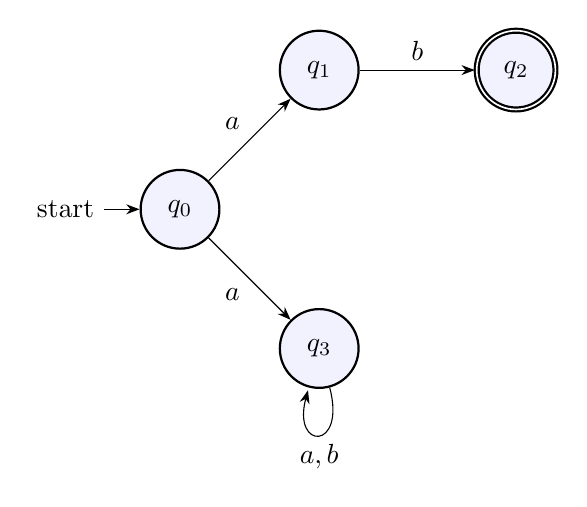
\begin{tikzpicture}[->, >=Stealth, node distance=2.5cm, every state/.style={thick, fill=blue!5, minimum size=1cm}]
    \node[state, initial] (q0) {$q_0$};
    \node[state] (q1) [above right of=q0] {$q_1$};
    \node[state, accepting] (q2) [right of=q1] {$q_2$};
    \node[state] (q3) [below right of=q0] {$q_3$};

    \path (q0) edge node[above left] {$a$} (q1)
          (q0) edge node[below left] {$a$} (q3)
          (q1) edge node[above] {$b$} (q2)
          (q3) edge [loop below] node {$a,b$} ();
\end{tikzpicture}
\end{center}

In this NFA, on input $a$ from state $q_0$, the machine has \textbf{two choices}: go to $q_1$ or $q_3$. On input $ab$, one branch ($q_0 \to q_1 \to q_2$) reaches the accepting state $q_2$, so the NFA accepts.

%-------------------------------------------------------------------------------
\subsection{NTM Formal Definition}

\begin{notebox}{Analogy: The Choose-Your-Own-Adventure Machine}
A deterministic TM is like reading a book: page 1 leads to page 2 leads to page 3. Linear, no choices.

A nondeterministic TM is like a choose-your-own-adventure book: page 10 might say ``To fight the dragon, turn to page 40. To run away, turn to page 55.'' The NTM ``reads'' every branch simultaneously. If ANY branch reaches ``The End --- You Win!'' (the accept state), the whole book is ``won.''

In our formal world: ``page'' = configuration; ``turn to page X'' = one possible transition; ``The End --- You Win'' = accept state $t$; ``winning'' = accepting.
\end{notebox}

\begin{definitionbox}{Nondeterministic Turing Machine (NTM) \kemark}

\textbf{Plain English:}
An NTM is exactly like a DTM except: where a DTM has exactly one possible move in each situation (one next state, one symbol to write, one direction), an NTM can have \textit{multiple} possible moves. The NTM ``tries all of them simultaneously'' and accepts if any choice sequence leads to acceptance.

\textbf{Formal Definition:}
An NTM is $M = (Q, \Sigma, \Gamma, \delta, s, t, r)$ where:
\fitmath{\delta: (Q \setminus \{t,r\}) \times \Gamma \to 2^{Q \times \Gamma \times \{-1, +1\}}}

\textbf{Comparison with DTM:}
\begin{center}
\begin{tabular}{lll}
\toprule
& \textbf{DTM} & \textbf{NTM} \\
\midrule
Transition returns & \textbf{one} triple $(q', b, d)$ & a \textbf{set} of triples \\
Domain & $(Q \setminus \{t,r\}) \times \Gamma$ & $(Q \setminus \{t,r\}) \times \Gamma$ (same!) \\
Range & $Q \times \Gamma \times \{-1,+1\}$ & $2^{Q \times \Gamma \times \{-1,+1\}}$ (power set!) \\
\# of next configs & Exactly 1 & 0, 1, 2, or more \\
\bottomrule
\end{tabular}
\end{center}

\textbf{Breaking Down the Notation:}
\begin{itemize}[nosep]
\item $2^{Q \times \Gamma \times \{-1,+1\}}$ = the power set (set of all subsets) of $Q \times \Gamma \times \{-1,+1\}$
\item This means $\delta(q, a)$ returns a \textbf{set} of possible moves, not a single move
\item Each element $(q', b, d)$ in the set is one possible transition: go to $q'$, write $b$, move $d$
\item The set can be \textbf{empty}: $\delta(q, a) = \emptyset$ means no move available (the computation branch dies)
\item A DTM is a special case of an NTM where every $\delta(q, a)$ has exactly one element
\end{itemize}

\kt{An NTM's $\delta$ returns a SET of possible moves. A DTM is just an NTM where every set has exactly one element.}
\end{definitionbox}

%-------------------------------------------------------------------------------
\subsection{The Computation Tree}

\begin{notebox}{Analogy: A Family Tree of Computations}
Think of a family tree. The ``ancestor'' (root) is the initial configuration. Each ``generation'' represents one step. A person can have multiple ``children'' --- these are the multiple possible next configurations. Some branches die out (dead ends). Some branches end with ``famous descendants'' (accept states).

The question is: does this family tree contain \textit{any} famous descendant?

In our formal world: ``ancestor'' = initial configuration $\alpha_w$; ``children'' = successor configurations from nondeterministic transitions; ``famous descendant'' = a configuration with state $t$ (accept); ``the tree'' = the computation tree.
\end{notebox}

\begin{definitionbox}{Computation Tree \kemark}

\textbf{Plain English:}
The computation tree of an NTM $M$ on input $w$ is a tree where:
\begin{itemize}[nosep]
\item The root is the initial configuration (start state, input on tape, head at position 0).
\item Each node is a configuration $[q, \tau, \ell]$.
\item The children of a node are ALL possible successor configurations (one child per element of $\delta(q, \tau(\ell))$).
\item Leaves are configurations where either: the state is $t$ (accept), the state is $r$ (reject), or $\delta(q, a) = \emptyset$ (dead end).
\end{itemize}

\textbf{Key properties:}
\begin{itemize}[nosep]
\item The tree can be \textbf{infinite} (if some branches loop forever and never reach $t$, $r$, or a dead end).
\item The tree can have different \textbf{branching factors} at different nodes (depends on $|\delta(q, a)|$).
\item A DTM's ``computation tree'' is just a single path (a chain, not a tree) because each node has exactly one child.
\end{itemize}

\kt{The computation tree shows ALL possible computations of an NTM on a given input. Each path from root to leaf is one possible ``run'' of the machine.}
\end{definitionbox}

Let us draw a concrete computation tree.

\begin{examplebox}{{Computation Tree: NTM for ``contains 110'' with input 0110}}

(We will define this NTM fully in Section~\ref{sec:ntm110}; for now, accept that at certain points, the machine has two choices: ``keep scanning'' or ``start checking for 110.'')

\textbf{Input: 0110}

At each position where the NTM reads a 1, it can (1) skip the symbol and move right, or (2) start trying to match ``110'' starting here.

\begin{center}
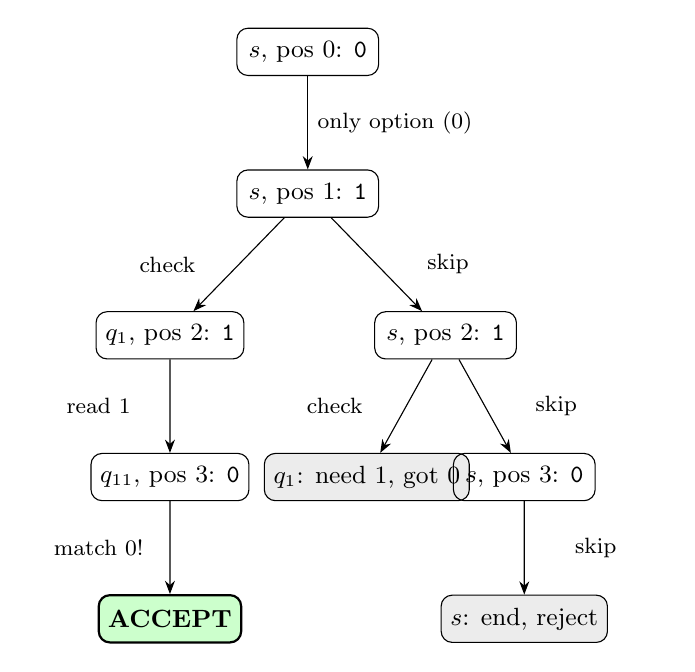
\begin{tikzpicture}[
    level distance=1.8cm,
    level 1/.style={sibling distance=6cm},
    level 2/.style={sibling distance=3.5cm},
    level 3/.style={sibling distance=2cm},
    every node/.style={draw, rounded corners, minimum width=1.8cm, minimum height=0.6cm, font=\small},
    edge from parent/.style={draw, ->, >=Stealth},
    accept/.style={fill=green!20, thick},
    reject/.style={fill=red!10},
    dead/.style={fill=gray!15}
]
\node {$s$, pos 0: \texttt{0}}
    child {
        node {$s$, pos 1: \texttt{1}}
        child {
            node {$q_1$, pos 2: \texttt{1}}
            child {
                node {$q_{11}$, pos 3: \texttt{0}}
                child {
                    node[accept] {\textbf{ACCEPT}}
                    edge from parent node[left, draw=none, font=\footnotesize] {match 0!}
                }
                edge from parent node[left, draw=none, font=\footnotesize] {read 1}
            }
            edge from parent node[left, draw=none, font=\footnotesize] {check}
        }
        child {
            node {$s$, pos 2: \texttt{1}}
            child {
                node[dead] {$q_1$: need 1, got 0}
                edge from parent node[left, draw=none, font=\footnotesize] {check}
            }
            child {
                node {$s$, pos 3: \texttt{0}}
                child {
                    node[dead] {$s$: end, reject}
                    edge from parent node[right, draw=none, font=\footnotesize] {skip}
                }
                edge from parent node[right, draw=none, font=\footnotesize] {skip}
            }
            edge from parent node[right, draw=none, font=\footnotesize] {skip}
        }
        edge from parent node[right, draw=none, font=\footnotesize] {only option (0)}
    };
\end{tikzpicture}
\end{center}

\textbf{Reading the tree:}
\begin{itemize}[nosep]
\item Root: state $s$, reading \texttt{0} at position 0. Only one transition for $\delta(s, 0)$: skip. No branching here.
\item At position 1 (reading \texttt{1}): \textbf{branch!} Left child checks for 110, right child skips.
\item Left branch from position 1: reads \texttt{1} (good, first match), then \texttt{1} (good, second match), then \texttt{0} (good, third match). \textbf{Accept!}
\item Right branches: various failures (mismatches or reaching end of input).
\end{itemize}

\kt{The NTM accepts \texttt{0110} because at least one branch of the computation tree reaches an accepting state. It does not matter that other branches fail.}
\end{examplebox}

%-------------------------------------------------------------------------------
\subsection{NTM Acceptance: The ``Exists'' Rule}

\begin{conceptbox}{How NTMs Accept \kemark}

\textbf{The rule is simple but must be stated precisely:}

An NTM $M$ \textbf{accepts} input $w$ if the computation tree of $M$ on $w$ \textbf{contains at least one accepting configuration} (i.e., a configuration where the state is $t$).

\fitmath{M \text{ accepts } w \iff \exists \text{ a path from the root to a node with state } t}

Equivalently: $M$ accepts $w$ if there exists a sequence of nondeterministic choices such that $M$ reaches $t$.

\textbf{Important consequences:}
\begin{itemize}[nosep]
\item \textbf{One accept branch suffices.} Even if 999 branches reject and 1 branch accepts, the NTM accepts.
\item \textbf{Reject requires ALL branches to reject (or die).} The NTM rejects $w$ only if \textit{no} branch of the computation tree ever reaches $t$.
\item \textbf{Looping branches do not help or hurt.} If some branches loop forever and no branch accepts, the NTM does NOT accept. But the tree might be infinite, making it unclear whether to ``wait longer'' or give up.
\end{itemize}

\textbf{The accept/reject asymmetry:}

\begin{center}
\begin{tabular}{ll}
\toprule
\textbf{To accept:} & $\exists$ at least one accepting branch \\
\textbf{To reject:} & $\forall$ branches either reject or die (no branch accepts) \\
\bottomrule
\end{tabular}
\end{center}

This asymmetry ($\exists$ for accept, $\forall$ for reject) is fundamental. It is why NTMs are great at \textit{verifying} things but not obviously great at \textit{refuting} things.
\end{conceptbox}

%-------------------------------------------------------------------------------
\subsection{Halting NTMs}

\begin{definitionbox}{Halting NTM \kemark}

\textbf{Plain English:}
A halting NTM is one where the computation tree is \textbf{finite} for every input. No branch loops forever. Every branch eventually reaches $t$, $r$, or a dead end.

\textbf{Formal:}
An NTM $M$ is \textbf{halting} if for every input $w \in \Sigma^*$, the computation tree of $M$ on $w$ is finite.

\textbf{Why this matters:}
\begin{itemize}[nosep]
\item A halting NTM is the NTM equivalent of a ``decider'' (total TM).
\item For a halting NTM, the computation tree has finitely many leaves. We can check whether any leaf is accepting, and if not, the machine rejects.
\item Halting NTMs \textbf{decide} languages (always accept or reject, never loop).
\end{itemize}

\kt{A halting NTM has a finite computation tree on every input. This means it always terminates --- every branch eventually reaches accept, reject, or dead end.}
\end{definitionbox}

%-------------------------------------------------------------------------------
\subsection{The 5 Definitions of NTM Acceptance (Exercise 3)}

Exercise 3 from the problem set gives 5 proposed definitions of what it means for a halting NTM to accept in time $T$. Only one is correct. Understanding \textbf{why} each wrong one is wrong builds deep intuition about NTM semantics.

\begin{conceptbox}{Exercise 3: Which Definition is Correct? \kemark}

\textbf{Setup:} $M$ is a halting NTM, $w$ is an input, $T \in \mathbb{N}$.

\medskip
\textbf{Definition 1:} ``For all computations of $M(w)$, $M$ halts in at most $T$ steps in an accepting state.''

\textcolor{red}{\textbf{WRONG.}} This requires ALL branches to accept within $T$ steps. But NTM acceptance only needs ONE branch to accept. This definition turns acceptance from $\exists$ into $\forall$.

\medskip
\textbf{Definition 2:} ``For all computations of $M(w)$, $M$ halts in at most $T$ steps.''

\textcolor{red}{\textbf{WRONG.}} This says all branches halt within $T$ steps, but says nothing about \textit{accepting}. A machine where all branches reject in 1 step would satisfy this --- but it should not be said to ``accept in time $T$''.

\medskip
\textbf{Definition 3:} ``There exists a computation of $M(w)$ that halts in at most $T$ steps in an accepting state.''

\textcolor{green!60!black}{\textbf{CORRECT!}} This captures exactly the NTM semantics: there EXISTS a branch that (a) reaches state $t$ (accepting) and (b) does so within $T$ steps.

\medskip
\textbf{Definition 4:} ``There exists a computation of $M(w)$ that halts in at most $T$ steps.''

\textcolor{red}{\textbf{WRONG.}} Same problem as Definition 2: says nothing about accepting. There might exist a computation that halts quickly in a \textit{rejecting} state. This does not mean the NTM accepts.

\medskip
\textbf{Definition 5:} ``The number of steps performed during exploration of the computation tree (BFS) is at most $T$.''

\textcolor{red}{\textbf{WRONG.}} This conflates the \textit{simulation} cost (BFS of the tree) with the NTM's own time. The BFS might take exponentially many steps even if the NTM's branches are short. This measures the simulator's time, not the NTM's time.

\medskip
\textbf{Summary of the pattern:}

\begin{center}
\begin{tabular}{clcl}
\toprule
\# & Quantifier & Halts/Accepts? & Verdict \\
\midrule
1 & $\forall$ & accepts in $\leq T$ & Wrong (too strong: demands ALL accept) \\
2 & $\forall$ & halts in $\leq T$ & Wrong (halts $\neq$ accepts) \\
3 & $\exists$ & accepts in $\leq T$ & \textbf{Correct!} \\
4 & $\exists$ & halts in $\leq T$ & Wrong (halts $\neq$ accepts) \\
5 & BFS-based & --- & Wrong (measures simulator, not NTM) \\
\bottomrule
\end{tabular}
\end{center}

\kt{NTM acceptance uses $\exists$ (not $\forall$) and requires reaching state $t$ (not just halting). Only definition 3 gets both right: ``there exists a computation that halts in an accepting state within $T$ steps.''}
\end{conceptbox}

%-------------------------------------------------------------------------------
\subsection{Constructing NTMs: ``Contains 110''} \label{sec:ntm110}

Now let us build our running example NTM from scratch.

\begin{notebox}{Analogy: The Substring Spotter}
Imagine you are reading a long string of digits and you need to find whether ``110'' appears anywhere. A \textbf{deterministic} approach: scan from left to right, keep track of how much of ``110'' you have matched so far (a small state machine).

A \textbf{nondeterministic} approach: at every position, \textit{guess} ``maybe 110 starts here'' and check. If your guess is right at any position, accept. This is simpler to design because you do not need the bookkeeping of partial matches.

In our formal world: ``guess'' = nondeterministic choice; ``check'' = deterministic verification; ``guess is right at any position'' = some branch of the computation tree accepts.
\end{notebox}

\begin{definitionbox}{{NTM for $L_{110} = \{w \in \{0,1\}^* \mid w \text{ contains } 110\}$} \kemark}

\textbf{The states:}
\begin{itemize}[nosep]
\item $s$ = ``scanning'' --- have not decided where 110 starts yet
\item $q_1$ = ``matched first 1'' --- guessed that 110 starts, seen the first 1
\item $q_{11}$ = ``matched 11'' --- seen two 1s, need a 0 next
\item $t$ = accept (found 110)
\item $r$ = reject
\end{itemize}

\textbf{Input alphabet:} $\Sigma = \{0, 1\}$. \textbf{Tape alphabet:} $\Gamma = \{0, 1, \sqcup\}$.

\textbf{Transition function:}

\begin{center}
\begin{tabular}{lll}
\toprule
State & Read & $\delta$ (set of possible moves) \\
\midrule
$s$ & $0$ & $\{(s, 0, +1)\}$ \quad (only option: skip, move right) \\
$s$ & $1$ & $\{(s, 1, +1),\ (q_1, 1, +1)\}$ \quad (\textbf{TWO options}: skip OR start matching) \\
$s$ & $\sqcup$ & $\{(r, \sqcup, +1)\}$ \quad (reached end without finding 110: reject) \\
$q_1$ & $1$ & $\{(q_{11}, 1, +1)\}$ \quad (second 1 found, continue) \\
$q_1$ & $0$ & $\{(r, 0, +1)\}$ \quad (needed 1, got 0: this branch fails) \\
$q_1$ & $\sqcup$ & $\{(r, \sqcup, +1)\}$ \quad (input ended too early: fail) \\
$q_{11}$ & $0$ & $\{(t, 0, +1)\}$ \quad (found the 0 after 11: \textbf{ACCEPT!}) \\
$q_{11}$ & $1$ & $\{(r, 1, +1)\}$ \quad (needed 0, got 1: fail) \\
$q_{11}$ & $\sqcup$ & $\{(r, \sqcup, +1)\}$ \quad (input ended: fail) \\
\bottomrule
\end{tabular}
\end{center}

\textbf{The key nondeterministic transition:} $\delta(s, 1) = \{(s, 1, +1),\ (q_1, 1, +1)\}$

This says: ``When in the scanning state and reading a 1, I have two choices:
\begin{enumerate}[nosep]
\item Stay in $s$ (skip this 1, maybe 110 starts later) and move right.
\item Go to $q_1$ (guess that 110 starts here, begin checking) and move right.''
\end{enumerate}

All other transitions are deterministic (sets with exactly one element).
\end{definitionbox}

\begin{center}
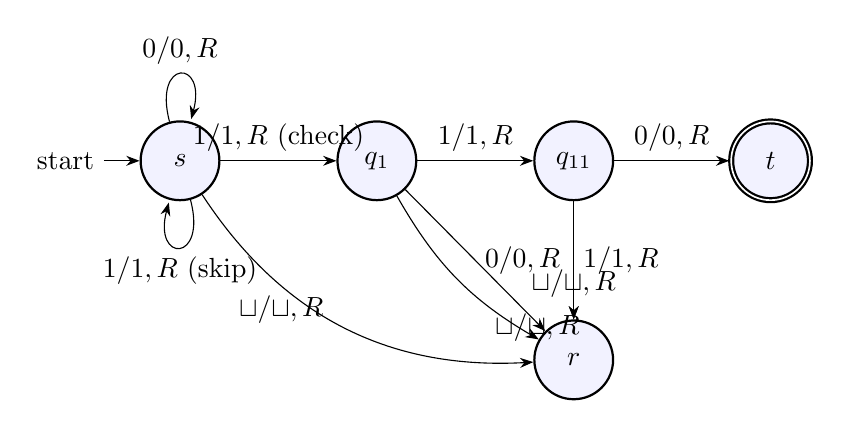
\begin{tikzpicture}[->, >=Stealth, node distance=2.5cm, every state/.style={thick, fill=blue!5, minimum size=1cm}]
    \node[state, initial] (s) {$s$};
    \node[state] (q1) [right of=s] {$q_1$};
    \node[state] (q11) [right of=q1] {$q_{11}$};
    \node[state, accepting] (t) [right of=q11] {$t$};
    \node[state] (r) [below=1.5cm of q11] {$r$};

    \path (s) edge [loop above] node {$0/0,R$} (s)
          (s) edge [loop below] node[below] {$1/1,R$ (skip)} (s)
          (s) edge node[above] {$1/1,R$ (check)} (q1)
          (s) edge [bend right=30] node[below, pos=0.3] {$\sqcup/\sqcup,R$} (r)
          (q1) edge node[above] {$1/1,R$} (q11)
          (q1) edge node[right] {$0/0,R$} (r)
          (q1) edge [bend right=15] node[below right, pos=0.7] {$\sqcup/\sqcup,R$} (r)
          (q11) edge node[above] {$0/0,R$} (t)
          (q11) edge node[right] {$1/1,R$} (r)
          (q11) edge node[below] {$\sqcup/\sqcup,R$} (r);
\end{tikzpicture}
\end{center}

Note the two arrows from $s$ labeled $1/1,R$: one loops back to $s$ (skip), the other goes to $q_1$ (check). This is the nondeterminism.

%-------------------------------------------------------------------------------
\subsubsection{Full Trace on Accepting Input: \texttt{0110}}

\begin{examplebox}{{Trace: NTM for ``contains 110'' on input 0110}}

\textbf{Input:} \texttt{0110}. We expect acceptance (110 starts at position 1).

We trace the full computation tree. Each node is a configuration; we branch whenever there is a nondeterministic choice.

\textbf{Step 0:} Config $[s,\ \underline{0}110\sqcup,\ 0]$. Read $0$ in state $s$.
\begin{itemize}[nosep]
\item $\delta(s, 0) = \{(s, 0, +1)\}$ --- only one option. Move right, stay in $s$.
\end{itemize}

\textbf{Step 1:} Config $[s,\ 0\underline{1}10\sqcup,\ 1]$. Read $1$ in state $s$.
\begin{itemize}[nosep]
\item $\delta(s, 1) = \{(s, 1, +1),\ (q_1, 1, +1)\}$ --- \textbf{TWO options. Branch!}
\end{itemize}

\textbf{Branch A (skip):} Stay in $s$, move right.

\quad \textbf{Step 2A:} Config $[s,\ 01\underline{1}0\sqcup,\ 2]$. Read $1$ in state $s$.
\begin{itemize}[nosep]
\item Branch again: $\delta(s, 1) = \{(s, 1, +1),\ (q_1, 1, +1)\}$
\end{itemize}

\quad \textbf{Branch A1 (skip again):} $[s,\ 011\underline{0}\sqcup,\ 3]$. Read $0$, $\delta(s,0) = \{(s,0,+1)\}$. Move right.

\quad\quad $[s,\ 0110\underline{\sqcup},\ 4]$. Read $\sqcup$, $\delta(s, \sqcup) = \{(r, \sqcup, +1)\}$. \textbf{Reject.} (Scanned entire input without ever guessing.)

\quad \textbf{Branch A2 (check from position 2):} $[q_1,\ 011\underline{0}\sqcup,\ 3]$. Read $0$ in state $q_1$.

\quad\quad $\delta(q_1, 0) = \{(r, 0, +1)\}$. Needed a second 1, got 0. \textbf{Reject.}

\textbf{Branch B (check from position 1):} Go to $q_1$, move right.

\quad \textbf{Step 2B:} Config $[q_1,\ 01\underline{1}0\sqcup,\ 2]$. Read $1$ in state $q_1$.

\quad $\delta(q_1, 1) = \{(q_{11}, 1, +1)\}$. Second 1 found! Move to $q_{11}$.

\quad \textbf{Step 3B:} Config $[q_{11},\ 011\underline{0}\sqcup,\ 3]$. Read $0$ in state $q_{11}$.

\quad $\delta(q_{11}, 0) = \{(t, 0, +1)\}$. Found the 0 after 11! \textbf{ACCEPT!}

\bigskip
\textbf{Summary of all branches:}
\begin{center}
\begin{tabular}{llll}
\toprule
Branch & Choice sequence & Final state & Result \\
\midrule
A1 & skip at pos 1, skip at pos 2 & $r$ & Reject \\
A2 & skip at pos 1, check at pos 2 & $r$ & Reject (no 110 from pos 2) \\
B & check at pos 1 & $t$ & \textbf{Accept!} \\
\bottomrule
\end{tabular}
\end{center}

Since Branch B reaches $t$, the NTM \textbf{accepts} \texttt{0110}. The two rejecting branches are irrelevant.
\end{examplebox}

%-------------------------------------------------------------------------------
\subsubsection{Full Trace on Rejecting Input: \texttt{0010}}

\begin{examplebox}{{Trace: NTM for ``contains 110'' on input 0010}}

\textbf{Input:} \texttt{0010}. We expect rejection (no 110 substring).

\textbf{Step 0:} $[s,\ \underline{0}010\sqcup,\ 0]$. Read $0$. Only option: $(s, 0, +1)$. Move right.

\textbf{Step 1:} $[s,\ 0\underline{0}10\sqcup,\ 1]$. Read $0$. Only option: $(s, 0, +1)$. Move right.

\textbf{Step 2:} $[s,\ 00\underline{1}0\sqcup,\ 2]$. Read $1$. \textbf{Branch!}

\textbf{Branch A (skip):} $[s,\ 001\underline{0}\sqcup,\ 3]$. Read $0$. Only $(s, 0, +1)$. Move right.

\quad $[s,\ 0010\underline{\sqcup},\ 4]$. Read $\sqcup$. $(r, \sqcup, +1)$. \textbf{Reject.}

\textbf{Branch B (check from pos 2):} $[q_1,\ 001\underline{0}\sqcup,\ 3]$. Read $0$ in $q_1$.

\quad $\delta(q_1, 0) = \{(r, 0, +1)\}$. Needed second 1, got 0. \textbf{Reject.}

\textbf{All branches reject.} No branch reaches $t$. The NTM \textbf{rejects} \texttt{0010}.

Note: the only nondeterministic choice was at position 2 (reading the only 1 in the input). But starting to match ``110'' from position 2 fails immediately because the next symbol is 0, not 1. And skipping also fails because there are no more 1s to try.
\end{examplebox}

%-------------------------------------------------------------------------------
\subsection{Constructing NTMs: Composite Numbers (Guess and Verify)}

\begin{notebox}{Analogy: The Party Trick}
Someone gives you a number and asks ``Is this composite (not prime)?'' You need to prove it is. Instead of systematically testing all divisors (deterministic approach), you \textit{guess} two factors and multiply them. If the product matches the number, you have proven it is composite.

This is the ``guess and verify'' pattern: the NTM \textit{guesses} a certificate (the two factors) and then \textit{deterministically verifies} it.

In our formal world: ``guessing'' = nondeterministic phase; ``verifying'' = deterministic phase; ``certificate'' = the guessed factors $n_0, n_1 > 1$.
\end{notebox}

\begin{definitionbox}{{NTM for $L_{\text{comp}} = \{a^n \mid n \text{ is composite}\}$} \kemark}

\textbf{Plain English:}
The input is $n$ copies of the symbol $a$ (unary encoding of $n$). We accept if $n$ is composite (i.e., $n = n_0 \cdot n_1$ for some $n_0, n_1 > 1$).

\textbf{The NTM strategy (guess and verify):}

\textbf{Phase 1 (Nondeterministic): Guess $n_0$ and $n_1$.}
\begin{itemize}[nosep]
\item Nondeterministically guess two integers $n_0 > 1$ and $n_1 > 1$.
\item Concretely: write $n_0$ in unary on a work tape by nondeterministically deciding when to stop writing.
\item Similarly write $n_1$ on another work tape (or a different section of the same tape).
\end{itemize}

\textbf{Phase 2 (Deterministic): Verify $n_0 \cdot n_1 = n$.}
\begin{itemize}[nosep]
\item Deterministically compute $n_0 \times n_1$ (by repeated addition: add $n_0$ to itself $n_1$ times).
\item Check if the result equals $n$ (the length of the input).
\item If yes: accept. If no: reject.
\end{itemize}

\textbf{Why this works:}
\begin{itemize}[nosep]
\item If $n$ IS composite, there EXIST factors $n_0, n_1 > 1$ with $n_0 \cdot n_1 = n$. At least one nondeterministic branch will guess these factors. That branch's verification succeeds. The NTM accepts.
\item If $n$ is NOT composite (i.e., $n$ is prime or 0 or 1), NO factors $n_0, n_1 > 1$ exist with $n_0 \cdot n_1 = n$. Every branch's verification fails. The NTM rejects.
\end{itemize}

\kt{The ``guess and verify'' pattern: nondeterministically guess a solution (certificate), then deterministically check it. If the problem has a solution, some branch guesses it correctly. If not, all branches fail verification.}
\end{definitionbox}

\begin{examplebox}{Example: Composite Number NTM on $a^6$}

\textbf{Input:} $aaaaaa$ (6 copies of $a$). Is 6 composite? Yes, $6 = 2 \times 3$.

\textbf{Some branches of the computation tree:}
\begin{itemize}[nosep]
\item Branch ``guess $n_0=2, n_1=2$'': verify $2 \times 2 = 4 \neq 6$. \textbf{Reject.}
\item Branch ``guess $n_0=2, n_1=3$'': verify $2 \times 3 = 6 = 6$. \textbf{Accept!}
\item Branch ``guess $n_0=3, n_1=2$'': verify $3 \times 2 = 6 = 6$. \textbf{Accept!}
\item Branch ``guess $n_0=4, n_1=2$'': verify $4 \times 2 = 8 \neq 6$. \textbf{Reject.}
\item \ldots (many other branches, most reject)
\end{itemize}

Since at least one branch accepts (e.g., $n_0=2, n_1=3$), the NTM accepts $a^6$.

\textbf{On input $a^5$ (5 is prime):} Every branch guesses some $n_0, n_1 > 1$, but $n_0 \times n_1$ never equals 5 (since 5's only factorizations are $1 \times 5$ and $5 \times 1$, both involving 1, and we require both factors $> 1$). All branches reject. NTM rejects.
\end{examplebox}

%-------------------------------------------------------------------------------
\subsection{The Simulation Theorem: Every NTM Can Be Simulated by a DTM}

\begin{conceptbox}{NTM-to-DTM Simulation Theorem \kemark}

\textbf{Theorem:} For every NTM $M$, there exists a DTM $M'$ that outcome-simulates $M$.

\textbf{Plain English:} Nondeterminism does not let you decide new languages. Anything an NTM can decide, a DTM can also decide. Nondeterminism is a convenience, not extra power.

\textbf{Why this is surprising:} An NTM can explore exponentially many branches ``simultaneously.'' How can a single-path DTM match that? By exploring the branches \textbf{one at a time}, systematically.
\end{conceptbox}

%-------------------------------------------------------------------------------
\subsection{The BFS Simulation: How a DTM Simulates an NTM}

\begin{notebox}{Analogy: Exploring a Maze Level by Level}
Back to the maze analogy. The NTM ``clones'' itself at every fork. A DTM cannot clone. But it \textit{can} explore the maze \textbf{systematically}: check all paths of length 1, then all paths of length 2, then length 3, etc. This is \textbf{breadth-first search (BFS)}.

Why BFS and not DFS (depth-first)? Because some paths might be \textbf{infinite}. If you go deep down one infinite path (DFS), you will never come back to check the other paths. BFS guarantees that if there is an accepting configuration at depth $d$, you will find it after exploring all configurations up to depth $d$.

In our formal world: ``maze'' = computation tree; ``paths of length $d$'' = configurations reachable in $d$ steps; ``BFS'' = explore all configs at depth $d$ before any at depth $d+1$.
\end{notebox}

\begin{definitionbox}{{BFS Simulation Algorithm} \kemark}

\textbf{Plain English:}
The DTM $M'$ explores the NTM's computation tree level by level. At each level, it checks whether any configuration is accepting. If it finds one: accept. If an entire level has no successors: reject (the tree is exhausted). Otherwise, compute the next level and continue.

\textbf{Algorithm (with line-by-line comments):}
\begin{lstlisting}
Input: w                                  % The input string
Gamma_0 := {alpha_w}                      % Level 0: just the initial config [s, w, 0]
i := 0                                    % Current depth counter
LOOP:                                     % Main loop: explore one level per iteration
  if Gamma_i contains config with state t:  % Check: is any config at this level accepting?
    ACCEPT                                % Found an accepting config -- we are done!
  if Gamma_i = empty set:                 % Check: is this level empty?
    REJECT                                % Tree exhausted, no accept found anywhere
  Gamma_{i+1} := {}                       % Initialize the next level as empty
  for each config alpha in Gamma_i:       % Process each config at the current level
    for each (q',b,d) in delta(q, a):     % For each possible NTM transition from alpha
      add successor config to Gamma_{i+1} % Compute and store the resulting config
  i := i + 1                              % Advance to the next depth level
  GOTO LOOP                               % Continue the main loop
\end{lstlisting}

\textbf{Breaking down each component:}
\begin{itemize}[nosep]
\item $\alpha_w$ = the initial configuration $[s, w\sqcup\sqcup\cdots, 0]$ (start state, input on tape, head at 0)
\item $\Gamma_i$ = the set of ALL configurations reachable from $\alpha_w$ in exactly $i$ steps (one ``level'' of the tree)
\item ``contains config with state $t$'' = any $[t, \tau, \ell] \in \Gamma_i$
\item ``all successors'' = for each config $\alpha = [q, \tau, \ell] \in \Gamma_i$ and each $(q', b, d) \in \delta(q, \tau(\ell))$, compute the next configuration and add it to $\Gamma_{i+1}$
\item $\Gamma_i = \emptyset$ means no configurations exist at depth $i$. Since every branch has terminated (reached $t$, $r$, or dead end) before depth $i$, the tree is fully explored. If we never found an accept, reject.
\end{itemize}

\kt{BFS of the computation tree: explore all branches level by level. Accept if any config at any level is accepting. Reject if the tree is exhausted (a level is empty). BFS is essential --- DFS can get stuck in infinite branches.}
\end{definitionbox}

\begin{conceptbox}{Why BFS and Not DFS? \kemark}

This is a critical design choice. Let us see why DFS fails.

\begin{center}
\begin{tabular}{p{5.5cm}p{5.5cm}}
\toprule
\textbf{BFS (Breadth-First)} & \textbf{DFS (Depth-First)} \\
\midrule
Explores level 0, then 1, then 2, \ldots & Goes as deep as possible on one branch, then backtracks. \\[0.5em]
If accept exists at depth $d$, found after exploring levels $0, \ldots, d$. Guaranteed. & Might go infinitely deep on a non-accepting branch and \textbf{never find} the accepting branch! \\[0.5em]
\textbf{Correct:} finds accept if one exists at any finite depth. & \textbf{NOT correct:} can get stuck in infinite branches. \\
\bottomrule
\end{tabular}
\end{center}

\textbf{Concrete example of DFS failure:} Suppose the NTM's computation tree has two branches from the root: branch A loops forever (infinite depth), branch B accepts at depth 3. DFS might explore branch A first, going deeper and deeper, never returning. BFS hits depth 3 after finitely many steps and finds B's acceptance.

\kt{DFS can get stuck in infinite branches and miss accepting configurations that exist at finite depth. BFS explores all finite depths systematically and is guaranteed to find any accepting configuration.}
\end{conceptbox}

%-------------------------------------------------------------------------------
\subsection{Full Trace of BFS Simulation on ``Contains 110'' with Input \texttt{0110}}

\begin{examplebox}{{BFS Simulation Trace: DTM simulating the ``contains 110'' NTM on input 0110}}

We simulate the NTM from Section~\ref{sec:ntm110} using the BFS algorithm.

\textbf{Level 0:} $\Gamma_0 = \{[s,\ \underline{0}110,\ 0]\}$

Check: state is $s$, not $t$. No accept. $\Gamma_0 \neq \emptyset$, so continue.

Compute $\Gamma_1$: successors of $[s,\ \underline{0}110,\ 0]$.
\begin{itemize}[nosep]
\item $\delta(s, 0) = \{(s, 0, +1)\}$. One successor: $[s,\ 0\underline{1}10,\ 1]$.
\end{itemize}

\fitmath{\Gamma_1 = \{[s,\ 0\underline{1}10,\ 1]\}}

\rule{\linewidth}{0.4pt}

\textbf{Level 1:} $\Gamma_1 = \{[s,\ 0\underline{1}10,\ 1]\}$

Check: state is $s$, not $t$. No accept. Continue.

Compute $\Gamma_2$: successors of $[s,\ 0\underline{1}10,\ 1]$.
\begin{itemize}[nosep]
\item $\delta(s, 1) = \{(s, 1, +1),\ (q_1, 1, +1)\}$. \textbf{Two successors:}
  \begin{itemize}[nosep]
  \item $(s, 1, +1) \Rightarrow [s,\ 01\underline{1}0,\ 2]$ \quad (skipped the 1)
  \item $(q_1, 1, +1) \Rightarrow [q_1,\ 01\underline{1}0,\ 2]$ \quad (started checking for 110)
  \end{itemize}
\end{itemize}

\fitmath{\Gamma_2 = \{[s,\ 01\underline{1}0,\ 2],\ \ [q_1,\ 01\underline{1}0,\ 2]\}}

\rule{\linewidth}{0.4pt}

\textbf{Level 2:} $\Gamma_2 = \{[s,\ 01\underline{1}0,\ 2],\ [q_1,\ 01\underline{1}0,\ 2]\}$

Check both configs: states are $s$ and $q_1$. Neither is $t$. Continue.

Compute $\Gamma_3$:
\begin{itemize}[nosep]
\item From $[s,\ 01\underline{1}0,\ 2]$: $\delta(s, 1) = \{(s, 1, +1),\ (q_1, 1, +1)\}$.
  \begin{itemize}[nosep]
  \item $\Rightarrow [s,\ 011\underline{0},\ 3]$ and $[q_1,\ 011\underline{0},\ 3]$
  \end{itemize}
\item From $[q_1,\ 01\underline{1}0,\ 2]$: $\delta(q_1, 1) = \{(q_{11}, 1, +1)\}$.
  \begin{itemize}[nosep]
  \item $\Rightarrow [q_{11},\ 011\underline{0},\ 3]$
  \end{itemize}
\end{itemize}

\fitmath{\Gamma_3 = \{[s,\ 011\underline{0},\ 3],\ \ [q_1,\ 011\underline{0},\ 3],\ \ [q_{11},\ 011\underline{0},\ 3]\}}

\rule{\linewidth}{0.4pt}

\textbf{Level 3:} $\Gamma_3 = \{[s,\ 011\underline{0},\ 3],\ [q_1,\ 011\underline{0},\ 3],\ [q_{11},\ 011\underline{0},\ 3]\}$

Check all three: states are $s$, $q_1$, $q_{11}$. None is $t$. Continue.

Compute $\Gamma_4$:
\begin{itemize}[nosep]
\item From $[s,\ 011\underline{0},\ 3]$: $\delta(s, 0) = \{(s, 0, +1)\}$.
  \begin{itemize}[nosep]
  \item $\Rightarrow [s,\ 0110\underline{\sqcup},\ 4]$
  \end{itemize}
\item From $[q_1,\ 011\underline{0},\ 3]$: $\delta(q_1, 0) = \{(r, 0, +1)\}$.
  \begin{itemize}[nosep]
  \item $\Rightarrow [r,\ 0110\underline{\sqcup},\ 4]$ \quad (reject state --- this branch is done)
  \end{itemize}
\item From $[q_{11},\ 011\underline{0},\ 3]$: $\delta(q_{11}, 0) = \{(t, 0, +1)\}$.
  \begin{itemize}[nosep]
  \item $\Rightarrow [t,\ 0110\underline{\sqcup},\ 4]$ \quad $\leftarrow$ \textbf{State is $t$!}
  \end{itemize}
\end{itemize}

\fitmath{\Gamma_4 = \{[s,\ 0110\underline{\sqcup},\ 4],\ \ [r,\ 0110\underline{\sqcup},\ 4],\ \ [t,\ 0110\underline{\sqcup},\ 4]\}}

\rule{\linewidth}{0.4pt}

\textbf{Level 4:} $\Gamma_4$ contains $[t,\ 0110\underline{\sqcup},\ 4]$. State is $t$!

\textbf{ACCEPT!}

\medskip
\textbf{Summary:}
\begin{center}
\begin{tabular}{ccc}
\toprule
Level & \# of configs & Accept found? \\
\midrule
0 & 1 & No \\
1 & 1 & No \\
2 & 2 & No \\
3 & 3 & No \\
4 & 3 & \textbf{Yes!} \\
\bottomrule
\end{tabular}
\end{center}

The BFS simulator found the accepting configuration at level 4. The DTM simulation accepted \texttt{0110}, matching the NTM's answer.
\end{examplebox}

\begin{conceptbox}{Correctness of BFS Simulation \kemark}

Why does this BFS approach correctly simulate the NTM?

\textbf{1. If the NTM accepts $w$:}
There exists some branch that reaches $t$ at some depth $d$. The BFS will reach level $d$ and find this accepting configuration. The DTM accepts. (BFS is \textit{complete}: it visits every node at every finite depth.)

\textbf{2. If the NTM is halting and rejects $w$:}
The computation tree is finite (because $M$ is halting). Eventually, BFS will exhaust the tree ($\Gamma_i = \emptyset$ for some $i$) without finding an accept. The DTM rejects.

\textbf{3. If the NTM loops on $w$:}
The computation tree is infinite. BFS will keep exploring deeper and deeper levels, never exhausting the tree, never finding an accept. The DTM loops. This is correct behaviour for outcome-simulation: the NTM does not halt, and neither does the DTM.

\textbf{What This Proof Tells Us:}
The BFS simulation DTM perfectly mirrors the NTM's accept/reject behaviour. The cost is potentially exponential: if the NTM has branching factor $b$ and accepting depth $d$, BFS explores up to $O(b^d)$ configurations. But the \textit{correctness} is guaranteed.

\kt{BFS simulation is correct: it accepts when the NTM accepts, rejects when the halting NTM rejects, and loops when the NTM loops. The key property is that BFS eventually reaches every finite depth.}
\end{conceptbox}

\newpage

%###############################################################################
%###############################################################################
\section{More Robustness: The Doubly-Infinite Tape}
%###############################################################################
%###############################################################################

%-------------------------------------------------------------------------------
\subsection{What is a Doubly-Infinite Tape?}

\begin{notebox}{Analogy: The Number Line}
A standard TM's tape is like a ruler: it starts at 0 and extends infinitely to the right ($0, 1, 2, 3, \ldots$). You cannot go left of 0.

A doubly-infinite tape is like a \textbf{number line}: it extends infinitely in both directions ($\ldots, -3, -2, -1, 0, 1, 2, 3, \ldots$). The head can move left past position 0 to position $-1$, $-2$, etc.

In our formal world: ``ruler'' = standard tape ($\tau: \mathbb{N}_0 \to \Gamma$, positions $0, 1, 2, \ldots$); ``number line'' = doubly-infinite tape ($\tau: \mathbb{Z} \to \Gamma$, positions $\ldots, -2, -1, 0, 1, 2, \ldots$).
\end{notebox}

%-------------------------------------------------------------------------------
\subsection{Formal Definition}

\begin{definitionbox}{DTM with Doubly-Infinite Tape \kemark}

\textbf{Plain English:}
A doubly-infinite tape TM is identical to a standard TM except the tape has no left boundary. The head can move infinitely far left as well as right. Every cell to the left of the input is initially blank ($\sqcup$).

\textbf{Formal:}
A DTM with doubly-infinite tape is $M = (Q, \Sigma, \Gamma, \delta, s, t, r)$ where:
\begin{itemize}[nosep]
\item The tape content is $\tau: \mathbb{Z} \to \Gamma$ (indexed by \textbf{all integers}, not just $\mathbb{N}_0$).
\item The head position is $\ell \in \mathbb{Z}$ (can be negative).
\item Input $w = w_1 w_2 \cdots w_n$ is placed at positions $0, 1, \ldots, n-1$. All other positions (including negative ones) contain $\sqcup$.
\item A configuration is $[q, \tau, \ell]$ where $\tau: \mathbb{Z} \to \Gamma$ and $\ell \in \mathbb{Z}$.
\item The transition function is the same as a standard TM: $\delta: (Q \setminus \{t,r\}) \times \Gamma \to Q \times \Gamma \times \{-1, +1\}$.
\end{itemize}

\textbf{Breaking Down the Notation:}
\begin{itemize}[nosep]
\item $\mathbb{Z}$ = the integers: $\{\ldots, -2, -1, 0, 1, 2, \ldots\}$
\item $\tau: \mathbb{Z} \to \Gamma$ = every integer position has a tape symbol (most are $\sqcup$)
\item $\ell \in \mathbb{Z}$ = head can be at negative positions
\item The key difference from standard: $\tau: \mathbb{N}_0 \to \Gamma$ becomes $\tau: \mathbb{Z} \to \Gamma$, and $\ell \in \mathbb{N}_0$ becomes $\ell \in \mathbb{Z}$
\end{itemize}

\kt{A doubly-infinite tape TM uses $\mathbb{Z}$ instead of $\mathbb{N}_0$ for tape positions. The head can go left forever. Everything else is identical to a standard TM.}
\end{definitionbox}

%-------------------------------------------------------------------------------
\subsection{Singly-Infinite Simulates Doubly-Infinite}

\begin{notebox}{Analogy: Folding the Number Line}
Imagine you have a number line ($\ldots, -3, -2, -1, 0, 1, 2, 3, \ldots$) drawn on an infinitely long ribbon. You fold the ribbon at 0: the left half ($-1, -2, -3, \ldots$) stacks under the right half ($0, 1, 2, 3, \ldots$). Now you have a single strip with two layers. By marking which layer you are reading, you can access any position of the original number line.

In our formal world: ``ribbon'' = doubly-infinite tape; ``folding'' = interleaving positive and negative positions on one singly-infinite tape; ``layers'' = two tracks per cell; ``marking which layer'' = using the state to remember whether you are in the ``left half'' or ``right half.''
\end{notebox}

\begin{definitionbox}{{Construction: Singly-Infinite Simulates Doubly-Infinite} \kemark}

\textbf{The Idea:}
Interleave the positive and negative portions of the doubly-infinite tape onto a single singly-infinite tape using special markers.

\textbf{Tape layout (shifting approach):}
Use a marker $\ell$ at position 0 as a left boundary. The singly-infinite tape stores the doubly-infinite content shifted so that position $\ell$ is the current leftmost used cell.

\begin{itemize}[nosep]
\item Position 0 on the singly-infinite tape: the marker $\ell$ (left boundary indicator)
\item Positions 1, 2, 3, \ldots: the doubly-infinite tape's content starting from the leftmost cell used
\end{itemize}

\textbf{How head movement works:}
\begin{itemize}[nosep]
\item Moving right on the doubly-infinite tape: move right on the singly-infinite tape (straightforward).
\item Moving left on the doubly-infinite tape and not at the marker: move left on the singly-infinite tape (straightforward).
\item Moving left on the doubly-infinite tape at the marker: \textbf{shift} the entire tape contents one position to the right and insert a new blank cell at position 1. The head stays at position 1.
\end{itemize}

\textbf{Correctness:} Every cell of the doubly-infinite tape is accessible. The shifting operation creates room for negative positions as needed. The $\ell$ marker prevents the head from ``falling off'' the singly-infinite tape.
\end{definitionbox}

\begin{examplebox}{{Trace: Simulating a Doubly-Infinite Tape (Shifting Approach)}}

\textbf{Setup:} A doubly-infinite TM runs on input \texttt{ab}. Its computation moves the head left past position 0 (into negative positions) and writes an \texttt{X} at position $-1$.

\textbf{Singly-infinite simulator tape (initial):}
\begin{lstlisting}
Pos:  0     1     2     3     4     ...
Cell: [ell] [a]   [b]   [_]   [_]   ...
              ^
\end{lstlisting}
($\ell$ is the left boundary marker. Head is at position 1, representing doubly-infinite position 0.)

\textbf{Step 1:} The doubly-infinite machine moves left from position 0 to position $-1$.

On the singly-infinite tape, the head is at position 1. Moving left would put it at position 0, which is the $\ell$ marker. We need to go ``past'' it.

\textbf{Action: Shift everything right by 1.}
\begin{lstlisting}
Pos:  0     1     2     3     4     5     ...
Cell: [ell] [_]   [a]   [b]   [_]   [_]   ...
              ^
\end{lstlisting}
A new blank cell has been inserted at position 1 (representing doubly-infinite position $-1$). The head is now at this new cell.

\textbf{Step 2:} The doubly-infinite machine writes \texttt{X} at position $-1$.
\begin{lstlisting}
Pos:  0     1     2     3     4     5     ...
Cell: [ell] [X]   [a]   [b]   [_]   [_]   ...
              ^
\end{lstlisting}

The singly-infinite tape now correctly represents the doubly-infinite tape: \texttt{X} at position $-1$, \texttt{a} at position 0, \texttt{b} at position 1.

\textbf{Step 3:} If the machine now moves right, the head goes to position 2 (representing doubly-infinite position 0, which has \texttt{a}). No shifting needed.
\begin{lstlisting}
Pos:  0     1     2     3     4     5     ...
Cell: [ell] [X]   [a]   [b]   [_]   [_]   ...
                    ^
\end{lstlisting}

\textbf{Key observation:} Shifting is expensive ($O(n)$ per shift for tape of length $n$), but it is always correct. Each shift happens only when the head crosses the left boundary, which may happen $O(T)$ times over $T$ steps, giving a worst-case total of $O(T^2)$.
\end{examplebox}

%-------------------------------------------------------------------------------
\subsection{Doubly-Infinite Simulates Singly-Infinite}

\begin{definitionbox}{Construction: Doubly-Infinite Simulates Singly-Infinite \kemark}

\textbf{Plain English:}
This direction is easy. A singly-infinite tape is just the right half of a doubly-infinite tape. We use a special marker \texttt{\#} at position 0 of the doubly-infinite tape to mark the left boundary, and the machine never crosses it.

\textbf{Construction:}
\begin{itemize}[nosep]
\item Place \texttt{\#} at position $0$ on the doubly-infinite tape.
\item Place the input starting at position $1$: $w_1$ at position 1, $w_2$ at position 2, etc.
\item Modify the transition function: whenever the machine reads \texttt{\#} (the boundary marker), make it move right (simulating the standard TM's behaviour at the left edge --- the head cannot move further left).
\item All negative positions remain $\sqcup$ forever --- the machine never goes there.
\end{itemize}

\textbf{Why this works:} The standard TM's tape is positions $\{0, 1, 2, \ldots\}$. The doubly-infinite tape's positions $\{1, 2, 3, \ldots\}$ (right of the marker) perfectly simulate this. The marker at position 0 acts as the left boundary.
\end{definitionbox}

\begin{examplebox}{Trace: Doubly-Infinite Simulating Singly-Infinite}

\textbf{Singly-infinite machine's tape:} \texttt{a b} with head at position 0.

\textbf{Doubly-infinite simulator's tape:}
\begin{lstlisting}
Pos:  ... -2   -1    0     1     2     3     ...
Cell: ... [_]  [_]   [#]   [a]   [b]   [_]   ...
                            ^
\end{lstlisting}

The head is at position 1 (representing singly-infinite position 0).

If the singly-infinite machine tries to move left from position 0, the head would go to position 0 on the doubly-infinite tape and read \texttt{\#}. The modified transition says: ``Read \texttt{\#}? Move right.'' So the head bounces back to position 1. This correctly simulates the standard TM's left-boundary behavior (the head stays at position 0 if it tries to go left from there).
\end{examplebox}

\begin{conceptbox}{Both Directions Simulated: Equivalent Power}

We have shown:
\begin{enumerate}[nosep]
\item A singly-infinite tape TM can simulate a doubly-infinite tape TM (using shifting or interleaving).
\item A doubly-infinite tape TM can simulate a singly-infinite tape TM (using a boundary marker).
\end{enumerate}

Therefore, singly-infinite and doubly-infinite tape TMs decide \textbf{exactly the same languages}. Another robustness result!

\kt{Singly-infinite and doubly-infinite tape TMs are equivalent in power. Each can simulate the other. The doubly-infinite tape is more convenient but not more powerful.}
\end{conceptbox}

\newpage

%###############################################################################
%###############################################################################
\section{Summary and Key Takeaways}
%###############################################################################
%###############################################################################

%-------------------------------------------------------------------------------
\subsection{What We Learned}

\begin{conceptbox}{The Big Picture of Lecture 2}

\textbf{The central message:} Turing machines are \textbf{robust}. No matter how you upgrade them --- extra tapes, nondeterminism, stay direction, doubly-infinite tape --- they decide exactly the same set of languages. This robustness is the strongest evidence for the \textbf{Church-Turing Thesis}: TMs capture everything that is ``computable.''

\textbf{What we proved:}
\begin{enumerate}[nosep]
\item Stay direction TMs $\equiv$ standard TMs (simulate stay with right-then-left)
\item $k$-tape DTMs $\equiv$ 1-tape DTMs (interleave tapes; $O(T^2)$ slowdown)
\item NTMs $\equiv$ DTMs (BFS of computation tree)
\item Doubly-infinite tape TMs $\equiv$ singly-infinite tape TMs (shift or interleave; boundary marker)
\end{enumerate}

$\equiv$ here means ``decide exactly the same languages'' (can outcome-simulate each other).
\end{conceptbox}

%-------------------------------------------------------------------------------
\subsection{Key Concepts Recap}

\begin{center}
\begin{tabular}{p{3.5cm}p{8.5cm}}
\toprule
\textbf{Concept} & \textbf{One-Line Summary} \\
\midrule
Church-Turing Thesis & Everything intuitively computable is TM-computable. (Thesis, not theorem.) \\
Turing-completeness & A system can simulate every TM. (Java, Python, Excel, Minecraft, \ldots) \\
Robustness & Extensions do not increase TM power --- only convenience/speed. \\
Outcome-simulation & $M'$ simulates $M$ if they agree on halt/accept/reject for all inputs. \\
Stay direction & Head can stay put ($d=0$). Simulate: right-then-left with auxiliary state. \\
Multi-tape TM & $k$ tapes, $k$ heads, one shared state. Simulate: interleave tapes on one tape. \\
NTM & $\delta$ returns a SET of moves. Accepts if ANY branch accepts ($\exists$). \\
Computation tree & Tree of all possible NTM computations. Branches at nondeterministic choices. \\
BFS simulation & DTM explores NTM's tree level by level. Finds accept if one exists. \\
Doubly-infinite tape & Tape extends infinitely in both directions ($\mathbb{Z}$ instead of $\mathbb{N}_0$). \\
Guess and verify & NTM pattern: nondeterministically guess a certificate, deterministically check it. \\
\bottomrule
\end{tabular}
\end{center}

%-------------------------------------------------------------------------------
\subsection{Practical Guidelines for Exam Problems}

\begin{notebox}{When Building a Simulation}
\begin{enumerate}[nosep]
\item \textbf{Identify what is different.} What does the extension add that a standard TM does not have? (Extra tapes? Nondeterminism? Stay direction?)
\item \textbf{Design the encoding.} How will the standard TM represent the extension's extra information on its single tape? (Interleaved tuples? Head markers? Boundary markers?)
\item \textbf{Describe the simulation step.} For each step of the extended machine, what does the standard TM do? (Scan to find heads? Bounce back to simulate stay? BFS to explore branches?)
\item \textbf{Argue correctness.} Why does the simulation preserve the outcome? (Same accept/reject. Same halting behaviour.)
\item \textbf{Analyse cost.} How many steps of the standard TM per step of the extended machine? (Usually polynomial overhead.)
\end{enumerate}
\end{notebox}

\begin{notebox}{When Constructing an NTM}
\begin{enumerate}[nosep]
\item \textbf{Identify the ``guess.''} What is the nondeterministic choice? (Where does 110 start? What are the factors? Where to split?)
\item \textbf{Design the ``verify.''} Given the guess, how do you deterministically check it? (Match the pattern? Multiply and compare? Count and compare?)
\item \textbf{Write the transition function.} The nondeterministic transitions give sets with $>1$ element. Everything else is deterministic (sets with exactly 1 element).
\item \textbf{Draw the state diagram.} Use TikZ. Show the nondeterministic arrows clearly (two arrows from the same state with the same read symbol).
\item \textbf{Trace on accept AND reject inputs.} Show that the right branches accept (for inputs in $L$) and ALL branches reject (for inputs not in $L$).
\end{enumerate}
\end{notebox}

%-------------------------------------------------------------------------------
\subsection{Common Pitfalls}

\begin{conceptbox}{Common Mistakes to Avoid}
\begin{enumerate}[nosep]
\item \textbf{``Nondeterminism = randomness.''} No! NTM explores ALL branches; randomness picks ONE. The NTM accepts if ANY branch accepts, not ``with some probability.''

\item \textbf{``The Church-Turing Thesis is a theorem.''} No! It is a thesis (claim). It cannot be proved because ``intuitively computable'' has no formal definition. It could (in principle) be refuted.

\item \textbf{``Multi-tape TMs are more powerful.''} No! They are more convenient and faster, but they decide exactly the same languages. ``Power'' in computability = which languages are decidable.

\item \textbf{``NTMs accept if all branches accept.''} No! NTMs accept if $\exists$ (at least one) branch accepts. This is the single most tested misconception.

\item \textbf{``DFS works for simulating NTMs.''} Careful! DFS can get stuck in an infinite branch and never find the accepting branch. BFS is necessary for correctness (or iterative deepening DFS).

\item \textbf{``A DTM is not an NTM.''} Actually, a DTM IS a special case of an NTM where every $\delta(q,a)$ has exactly one element. The NTM model subsumes the DTM model.

\item \textbf{Forgetting auxiliary states in stay-simulation.} When you simulate stay with right-then-left, you MUST create fresh auxiliary states $q_L$. Otherwise the ``bouncing back'' step could collide with existing transitions.

\item \textbf{Forgetting head markers in multi-tape simulation.} When interleaving $k$ tapes on 1 tape, each cell stores $k$ symbols AND head-position markers. Without the markers, you cannot find where the heads are.
\end{enumerate}
\end{conceptbox}

%-------------------------------------------------------------------------------
\subsection{Quick Reference: Simulation Techniques}

\begin{center}
\begin{tabular}{p{2.8cm}p{2.8cm}p{6cm}}
\toprule
\textbf{Extension} & \textbf{Technique} & \textbf{Key Construction Detail} \\
\midrule
Stay ($d=0$) & Right-then-left & Auxiliary state $q_L$ per target state. Two moves simulate one stay. \\[0.3em]
$k$-tape & Interleave & Each cell stores $k$-tuple with hat markers. Scan twice per simulated step. $O(T^2)$ total. \\[0.3em]
Nondeterminism & BFS of tree & Maintain set $\Gamma_i$ of configs at depth $i$. Accept if any has state $t$. Reject if $\Gamma_i = \emptyset$. \\[0.3em]
Doubly-infinite (sim.\ by singly) & Shift / interleave & Shift tape right when head crosses left boundary marker. \\[0.3em]
Singly (sim.\ by doubly) & Boundary marker & Place \texttt{\#} at position 0. Never cross it. Positions $1, 2, \ldots$ simulate $0, 1, \ldots$ \\
\bottomrule
\end{tabular}
\end{center}

\kt{Every robustness proof follows the same pattern: (1) define the extension, (2) show a standard TM can simulate it via a clever encoding, (3) argue the simulation preserves accept/reject outcomes. Master this pattern and you can handle any variant the exam throws at you.}

\end{document}
